\documentclass[UTF8,a4paper,oneside]{book}
\usepackage{ctex}
\usepackage{framed}
\usepackage{amsthm}
\usepackage{geometry}
\usepackage{mathrsfs}
\geometry{left=1.414cm,right=1.314cm,top=2.414cm,bottom=2.315cm}
\usepackage{amsmath}
\usepackage{graphicx}
\usepackage{subfiles}
\linespread{1.5}
\usepackage{indentfirst}
\setlength{\parindent}{2em}

\setCJKmainfont[ItalicFont=FandolKai-Regular,BoldFont=STSongti-SC-Black]{STSong} 
\setCJKsansfont{FandolHei-Regular}
\setCJKmonofont{FandolFang-Regular}
\setCJKfamilyfont{kaiti}{FandolKai-Regular}
\setCJKfamilyfont{fang}{FandolFang-Regular}
\newcommand{\kaiti}{\CJKfamily{kaiti}}%\
\newcommand{\fang}{\CJKfamily{fang}}%
\setmainfont{Times New Roman}

\usepackage{physics}
\usepackage{paralist}

\usepackage{multicol}
\let\itemize\compactitem
\let\enditemize\endcompactitem
\let\enumerate\compactenum
\let\endenumerate\endcompactenum
\let\description\compactdesc
\let\enddescription\endcompactdesc
\usepackage{color}
\usepackage{fancyhdr} %调用宏包

% ---基本设置---

%设定页面的页眉页脚类型,$\LaTeX$内置了四种:empty、plain、headings及myheadings
\pagestyle{fancy}

%清除原页眉页脚样式
\fancyhf{} 

%R:页面右边;O:奇数页;\leftmark:表示“一级标题”
\fancyhead[CO]{\leftmark}

%L:页面左边;E:偶数页;\rightmark:表示“二级标题”
\fancyhead[CE]{\rightmark}

%C:页面中间
\fancyhead[CO, CE]{{\calligra The Homework For Chemical Engineering Thermodynamics}}

% 设置页脚,页眉的位置上也可以放置页码
\fancyhead[RO, LE]{$\cdot\ \textrm{\thepage} \ \cdot$}

% 设置页眉页脚横线及样式
%页眉线宽,设为0可以去页眉线
\renewcommand{\headrulewidth}{0.05em} 


%------------------------------设置字体大小------------------------%  
\newcommand{\chuhao}{\fontsize{42pt}{\baselineskip}\selectfont}     %初号  
\newcommand{\xiaochuhao}{\fontsize{36pt}{\baselineskip}\selectfont} %小初号  
\newcommand{\yihao}{\fontsize{28pt}{\baselineskip}\selectfont}      %一号  
\newcommand{\erhao}{\fontsize{21pt}{\baselineskip}\selectfont}      %二号  
\newcommand{\xiaoerhao}{\fontsize{18pt}{\baselineskip}\selectfont}  %小二号  
\newcommand{\sanhao}{\fontsize{15.75pt}{\baselineskip}\selectfont}  %三号  
\newcommand{\sihao}{\fontsize{14pt}{\baselineskip}\selectfont}       %四号  
\newcommand{\xiaosihao}{\fontsize{12pt}{\baselineskip}\selectfont}  %小四号  
\newcommand{\wuhao}{\fontsize{10.5pt}{\baselineskip}\selectfont}    %五号  
\newcommand{\xiaowuhao}{\fontsize{9pt}{\baselineskip}\selectfont}   %小五号  
\newcommand{\liuhao}{\fontsize{7.875pt}{\baselineskip}\selectfont}  %六号  
\newcommand{\qihao}{\fontsize{5.25pt}{\baselineskip}\selectfont}    %七号

\title{\textbf{《化工热力学》作业}}
\author{张博涵\quad 应化1903班\quad 学号:1912020312\\
{\calligra GitHub $:$ www.github.com/BHanZhang}\\
{\kaiti{起著重庄赤奋若}}}
\date{}
\usepackage{chemfig}
\usepackage{mathrsfs}
\usepackage{listings}
\usepackage{makeidx}
\makeindex
\usepackage{framed}
\usepackage{amsthm,amsmath,amssymb}
\usepackage{wrapfig}
\usepackage{graphicx}
\usepackage{mathrsfs}
\bibliographystyle{plain}
\usepackage{subfiles}
\usepackage{booktabs}
\usepackage{graphicx,times}
\usepackage{esint}
\usepackage{times}
\usepackage{subfigure}         
\usepackage{natbib}
\usepackage{amssymb,amsmath}
\usepackage{url}
\usepackage{geometry}
\usepackage{setspace}
\usepackage{subfigure}
\usepackage{booktabs}
\usepackage{array}
\usepackage{mhchem}
\usepackage{colortbl}
\usepackage{bm}
\usepackage{calligra}
\definecolor{myorgn}{rgb}{0.56,0.28,0.16}
\definecolor{myyelo}{rgb}{255,215,0}
\definecolor{mygray}{gray}{.9}
\definecolor{mypink}{rgb}{.99,.91,.95}
\definecolor{mycyan}{cmyk}{.3,0,0,0}
\definecolor{myblu}{RGB}{70,111,157}

\usepackage{environ}
\everymath{\displaystyle}  
\usepackage[breaklinks,colorlinks,linkcolor=black,citecolor=black,urlcolor=black]{hyperref}
\usepackage{tikz}



\definecolor{colora}{RGB}{210,185,152}
\definecolor{colorb}{rgb}{0.99,0.97,0.93}

\newcounter{problemname}
\setcounter{problemname}{0}
\newcounter{solutionname}
\setcounter{solutionname}{0}
\newcounter{tipname}
\setcounter{tipname}{0}
\usepackage{geometry}
\usepackage{lipsum}
\usepackage{newtxtext}
\usepackage{xcolor}
\usepackage{tcolorbox}

\tcbuselibrary{most}

% ------------------******-------------------
\newtcolorbox{ti}[2][]
{enhanced,breakable,
left=12pt,right=12pt,% 左右边距
coltitle=white, % 标题字体颜色
colbacktitle=colora, % 标题背景颜色
attach boxed title to top left={yshifttext=-1mm},
boxed title style={skin=enhancedfirst jigsaw,arc=1mm,bottom=0mm,boxrule=0mm},
boxrule=1pt, % 边框线宽
colback=colorb, % 文本框背景颜色
colframe=colora, % 框线颜色
sharp corners=northwest,
drop fuzzy shadow, % 可以选择是否设置阴影效果
title=\vspace{3mm}#2,
arc=1mm,
#1}

\newenvironment{problem}{\begin{ti}{\stepcounter{problemname}\Large\textbf{{\calligra{Question \arabic{problemname}}}}}}{\end{ti}\par}

% ------------------******-------------------

\usepackage[center]{titlesec}
\titleformat{\chapter}{\raggedright\Huge\bfseries}{\arabic{chapter}}{1em}{}
\titleformat{\section}{\raggedright\Large\bfseries}{\,\thesection\,}{1em}{}
\titleformat{\subsection}{\raggedright\large\bfseries}{\,\thesubsection\,}{1em}{}

\usepackage[strict]{changepage} 
\definecolor{formalshade}{rgb}{0.90,0.99,0.91} % 文本颜色
\definecolor{Green}{RGB}{74,124,42} % 文本框颜色
% ------------------******-------------------

% ------------------******-------------------
\newtcolorbox{answer}[2][]
{enhanced,breakable,
left=12pt,right=12pt,% 左右边距
coltitle=white, % 标题字体颜色
colbacktitle=Green, % 标题背景颜色
attach boxed title to top left={yshifttext=-1mm},
boxed title style={skin=enhancedfirst jigsaw,arc=1mm,bottom=0mm,boxrule=0mm},
boxrule=1pt, % 边框线宽
colback=formalshade, % 文本框背景颜色
colframe=Green, % 框线颜色
sharp corners=northwest,
drop fuzzy shadow, % 可以选择是否设置阴影效果
title=\vspace{3mm}#2,
arc=1mm,
#1}

% ------------------******-------------------

\newenvironment{solution}{\begin{answer}{\stepcounter{solutionname}\Large\textbf{{\calligra{Answer \arabic{solutionname}}}}}}{\end{answer}\par}




\definecolor{redshade}{rgb}{1.00,0.90,0.90}% 阴影颜色
\definecolor{LightCoral}{RGB}{204,22,58} % 文本框颜色
% ------------------******-------------------
\newtcolorbox{tpp}[2][]
{enhanced,breakable,
left=12pt,right=12pt,% 左右边距
coltitle=white, % 标题字体颜色
colbacktitle=LightCoral, % 标题背景颜色
attach boxed title to top left={yshifttext=-1mm},
boxed title style={skin=enhancedfirst jigsaw,arc=1mm,bottom=0mm,boxrule=0mm},
boxrule=1pt, % 边框线宽
colback=redshade, % 文本框背景颜色
colframe=LightCoral, % 框线颜色
sharp corners=northwest,
drop fuzzy shadow, % 可以选择是否设置阴影效果
title=\vspace{3mm}#2,
arc=1mm,
#1}

\newenvironment{tip}{\begin{tpp}{\stepcounter{tipname}\Large\textbf{{\calligra{Tip \arabic{tipname}}}}}}{\end{tpp}\par}

% ------------------******-------------------

\newcommand{\qd}[2]{\dfrac{{\rm{d}}#1}{{\rm{d}}#2}}
\newcommand{\pd}[2]{\dfrac{\partial #1}{\partial #2}}
\newcommand{\rpd}[3]{\pqty{\dfrac{\partial #1}{\partial #2}}_{#3}}
\newcommand{\wei}[1]{{\rm{d}}#1}
\newcommand\ssd{$^{\circ}\rm{C}$}


\definecolor{mygray}{gray}{.9}
\definecolor{mypink}{rgb}{.99,.91,.95}
\definecolor{mycyan}{cmyk}{.3,0,0,0}
\usepackage{environ}
\everymath{\displaystyle}  
\usepackage{tikz}
\begin{document}
\setmainfont{Times New Roman}
	\maketitle
	\tableofcontents
\chapter{2022年3月10日\quad 晴}
本次作业中的所有体积$V$均表示摩尔体积$V_{\rm{m}}$
\begin{problem}
	将下列纯物质经历的过程表示在$p-V$图上:
\begin{enumerate}
	\item 过热蒸汽等温冷凝为过冷液体
	\item 过冷液体等压加热成过热蒸汽
	\item 饱和蒸汽可逆绝热膨胀
	\item 饱和液体恒容加热
	\item 在临界点进行的恒温膨胀
\end{enumerate}
\end{problem}

\begin{solution}


\begin{wrapfigure}[8]{r}{17em} 

\vspace{-0.9cm}
	\begin{center}
\tikzset{every picture/.style={line width=0.75pt}} %set default line width to 0.75pt        

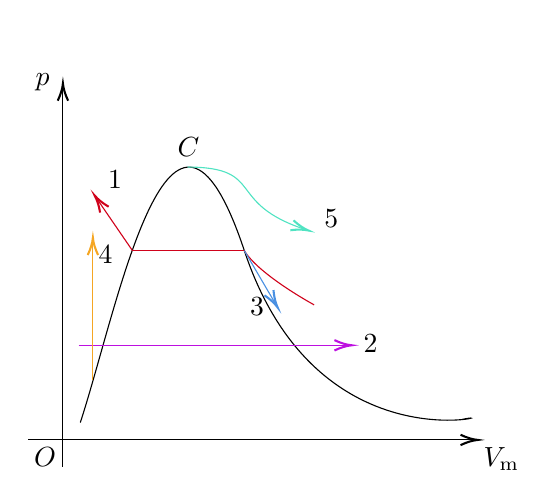
\begin{tikzpicture}[x=0.75pt,y=0.75pt,yscale=-1,xscale=1,scale=0.76]
%uncomment if require: \path (0,268); %set diagram left start at 0, and has height of 268

%Straight Lines [id:da9261157069712649] 
\draw    (33,258) -- (33,17) ;
\draw [shift={(33,15)}, rotate = 90] [color={rgb, 255:red, 0; green, 0; blue, 0 }  ][line width=0.75]    (10.93,-3.29) .. controls (6.95,-1.4) and (3.31,-0.3) .. (0,0) .. controls (3.31,0.3) and (6.95,1.4) .. (10.93,3.29)   ;
%Straight Lines [id:da40223898000413905] 
\draw    (11,241) -- (294,241) ;
\draw [shift={(296,241)}, rotate = 180] [color={rgb, 255:red, 0; green, 0; blue, 0 }  ][line width=0.75]    (10.93,-3.29) .. controls (6.95,-1.4) and (3.31,-0.3) .. (0,0) .. controls (3.31,0.3) and (6.95,1.4) .. (10.93,3.29)   ;
%Curve Lines [id:da8517089812043679] 
\draw    (44,230) .. controls (68,157) and (101,-20) .. (148,121) .. controls (195,262) and (320,221) .. (286,228) ;
%Straight Lines [id:da67833771454015] 
\draw [color={rgb, 255:red, 208; green, 2; blue, 27 }  ,draw opacity=1 ]   (77.09,121) -- (148,121) ;
%Curve Lines [id:da6846526882075424] 
\draw [color={rgb, 255:red, 208; green, 2; blue, 27 }  ,draw opacity=1 ]   (148,121) .. controls (157.25,136.37) and (192.25,155.37) .. (192.25,155.37) ;
%Straight Lines [id:da5556624828381672] 
\draw [color={rgb, 255:red, 208; green, 2; blue, 27 }  ,draw opacity=1 ]   (77.09,121) -- (54.22,87.65) ;
\draw [shift={(53.09,86)}, rotate = 55.56] [color={rgb, 255:red, 208; green, 2; blue, 27 }  ,draw opacity=1 ][line width=0.75]    (10.93,-3.29) .. controls (6.95,-1.4) and (3.31,-0.3) .. (0,0) .. controls (3.31,0.3) and (6.95,1.4) .. (10.93,3.29)   ;
%Straight Lines [id:da21149857233074754] 
\draw [color={rgb, 255:red, 189; green, 16; blue, 224 }  ,draw opacity=1 ]   (43,181) -- (214.06,181) ;
\draw [shift={(216.06,181)}, rotate = 180] [color={rgb, 255:red, 189; green, 16; blue, 224 }  ,draw opacity=1 ][line width=0.75]    (10.93,-3.29) .. controls (6.95,-1.4) and (3.31,-0.3) .. (0,0) .. controls (3.31,0.3) and (6.95,1.4) .. (10.93,3.29)   ;
%Straight Lines [id:da9678508805332595] 
\draw [color={rgb, 255:red, 74; green, 144; blue, 226 }  ,draw opacity=1 ]   (148,121) -- (168.15,155.38) ;
\draw [shift={(169.16,157.1)}, rotate = 239.63] [color={rgb, 255:red, 74; green, 144; blue, 226 }  ,draw opacity=1 ][line width=0.75]    (10.93,-3.29) .. controls (6.95,-1.4) and (3.31,-0.3) .. (0,0) .. controls (3.31,0.3) and (6.95,1.4) .. (10.93,3.29)   ;
%Straight Lines [id:da42681060344663924] 
\draw [color={rgb, 255:red, 245; green, 166; blue, 35 }  ,draw opacity=1 ]   (52,203) -- (52,114.85) ;
\draw [shift={(52,112.85)}, rotate = 90] [color={rgb, 255:red, 245; green, 166; blue, 35 }  ,draw opacity=1 ][line width=0.75]    (10.93,-3.29) .. controls (6.95,-1.4) and (3.31,-0.3) .. (0,0) .. controls (3.31,0.3) and (6.95,1.4) .. (10.93,3.29)   ;
%Curve Lines [id:da3137222686480874] 
\draw [color={rgb, 255:red, 80; green, 227; blue, 194 }  ,draw opacity=1 ]   (112,68) .. controls (162.1,68.22) and (135.16,90.77) .. (187.01,107.71) ;
\draw [shift={(188.61,108.22)}, rotate = 197.47] [color={rgb, 255:red, 80; green, 227; blue, 194 }  ,draw opacity=1 ][line width=0.75]    (10.93,-3.29) .. controls (6.95,-1.4) and (3.31,-0.3) .. (0,0) .. controls (3.31,0.3) and (6.95,1.4) .. (10.93,3.29)   ;

% Text Node
\draw (14,7.4) node [anchor=north west][inner sep=0.75pt]    {$\mathnormal{p}$};
% Text Node
\draw (298,244.4) node [anchor=north west][inner sep=0.75pt]    {$V_{\mathrm{m}}$};
% Text Node
\draw (13,244.4) node [anchor=north west][inner sep=0.75pt]    {$O$};
% Text Node
\draw (60,68.4) node [anchor=north west][inner sep=0.75pt]    {$1$};
% Text Node
\draw (222,172.4) node [anchor=north west][inner sep=0.75pt]    {$2$};
% Text Node
\draw (150,149.4) node [anchor=north west][inner sep=0.75pt]    {$3$};
% Text Node
\draw (54,116.25) node [anchor=north west][inner sep=0.75pt]    {$4$};
% Text Node
\draw (197,93.4) node [anchor=north west][inner sep=0.75pt]    {$5$};
% Text Node
\draw (104,47.4) node [anchor=north west][inner sep=0.75pt]    {$C$};
\end{tikzpicture}
        \caption{$p-V$相图}
        \label{fig1-1}
	\end{center}
\end{wrapfigure}
此题答案如右图所示:
\begin{enumerate}
	\item 右侧为过热蒸汽区,左侧为过冷液体区,在冷凝过程中等温变化(1)。
	\item 左侧为过冷液体区,右侧为过热蒸汽区,等压加热,即压力不变(2)。
	\item 饱和蒸汽可逆绝热膨胀,此时$TV^{\gamma-1} = const.$,其中$\gamma = \dfrac{C_{p}}{C_{V}}$为绝热指数。很明显由于膨胀导致的$\Delta V >0$,使得$\Delta T<0$,从而温度下降(3)。
	\item 饱和液体恒容加热,从$p-V$相图上恒容,即竖直向上(4)。
	\item 在临界点进行的恒温膨胀,即沿$T = T_{c}$线进行膨胀(5)。
\end{enumerate}
\end{solution}

\begin{problem}

	在4L的刚性容器中装有50$^{\circ}\rm{C}$、2kg水的饱和气液混合物,已知50$^{\circ}\rm{C}$时水的饱和液相体积$V^{sl}=1.0121\rm{cm}^{3}\cdot \rm{g}^{-1}$,饱和气相体积$V^{sv}=12032\rm{cm}^{3}\cdot\rm{g}^{-1}$。现在将水慢慢加热,使得饱和气液混合物变成了单相,问此单相是什么?如果将容器换为400L,最终答案是什么?
\end{problem}

\begin{solution}
\begin{enumerate}
	\item 因为是刚性容器,所以加热过程为等容变化,因此随着温度增高,压力也会增高,在$p-V$相图上相点向上移动,一直达到泡点线,相变为单液相;继续加热,相点继续向上移动,达到超临界流体区,相变为超临界流体。
	\item 如果增大容器容积,那么该体系在$p-V$相图上相点向右移动,此时加热,相点向上移动,一直达到露点线,相变为单汽相;继续加热,相点继续向上移动,达到超临界流体区,相变为超临界流体。
\end{enumerate}
\end{solution}
\begin{problem}
	试分别用(1)Van der Walls,(2)R-K方程计算273.15K时将$\ce{CO2}$压缩到比体积为550.1cm$^{3}\cdot$mol$^{-1}$所需要的压力。实验值为3.090MPa。已知$\ce{CO2}$的临界参数和偏心因子为:$T_c$=304.2K、$p_c$=7.376MPa、$\omega$=0.225
\end{problem}
\begin{solution}
	\begin{enumerate}
		\item 使用Van der Walls Eq.先计算Van der Walls常数:
		\begin{equation*}
			a = \dfrac{27}{64}\dfrac{R^{2}T_{c}^{2}}{p_{c}} = \dfrac{27}{64}\times\dfrac{8.314^{2}\times 304.2^{2}}{7.376}\rm{Pa}\cdot \rm{m}^{6}\cdot\rm{Mmol}^{-2}=153737\rm{Pa}\cdot \rm{m}^{6}\cdot\rm{Mmol}^{-2}
		\end{equation*}
		\begin{equation*}
			b = \dfrac{RT_{c}}{8p_{c}} = \dfrac{8.314\times 304.2}{8\times 7.376}\rm{m}^{3}\cdot\rm{Mmol}^{-1}= 42.86\rm{m}^{3}\cdot\rm{Mmol}^{-1}
		\end{equation*}
		然后直接带入方程:
		\begin{equation}
			p = \dfrac{RT}{V-b}-\dfrac{a}{V^{2}} = \dfrac{8.314\cdot 273.15}{550.1-42.86}-\dfrac{153737}{550.1^{2}}\rm{Mpa}=3.969\rm{Mpa}
		\label{eq1-1}
		\end{equation}
		\item 使用R-K Eq.先计算$a$、$b$:
		\begin{equation*}
			a = 0.42748\dfrac{R^{2}T_{c}^{2.5}}{p_{c}} = 0.42748\times\dfrac{8.314^{2}\times 304.2^{2.5}}{7.376}\rm{Pa}\cdot \rm{K}^{0.5}\cdot\rm{m}^{6}\cdot\rm{Mmol}^{-2}=6465661\rm{Pa}\cdot \rm{K}^{0.5}\cdot\rm{m}^{6}\cdot\rm{Mmol}^{-2}
		\end{equation*}
		\begin{equation*}
			b = 0.08664\times\dfrac{RT_{c}}{p_{c}} = 0.08664\times\dfrac{8.314\times 304.2}{ 7.376}\rm{m}^{3}\cdot\rm{Mmol}^{-1}=29.71\rm{m}^{3}\cdot\rm{Mmol}^{-1}
		\end{equation*}
		然后直接带入方程:
		\begin{equation}
			\begin{aligned}
			p = \dfrac{RT}{V-b}-\dfrac{a}{T^{0.5}V(V+b)} &=\dfrac{8.314\cdot 273.15}{550.1-29.71}-\dfrac{6465661}{273.15^{0.5}\times 550.1(550.1+29.71)} \rm{MPa}\\&= 3.137\rm{MPa}
			\end{aligned}
			\label{eq1-2}
		\end{equation}
	\end{enumerate}
\end{solution}
\begin{problem}
	使用下述方法计算1kmol甲烷贮存在体积为0.1246$\rm{m}^{3}$、温度为50$^{\circ}\rm{C}$的容器中产生的压力:(1)理想气体方程;(2)R-K方程
\end{problem}
\begin{solution}
\begin{enumerate}
	\item 使用理想气体状态方程:
	直接带入理想气体状态方程啊:
	\begin{equation*}
		p = \dfrac{nRT}{V} = \dfrac{1\times 10^{3}\times 8.314\times(50+273.15)}{0.1246}\rm{Pa} = 21.56\rm{MPa}
	\end{equation*}
	\item 使用R-K Eq.先计算$a$、$b$,首先查得甲烷的$T_{c} = 190.6$K、$p_{c} = 4.600$MPa。
		\begin{equation*}
			a = 0.42748\dfrac{R^{2}T_{c}^{2.5}}{p_{c}} = 0.42748\times\dfrac{8.314^{2}\times  190.6^{2.5}}{4.600}\rm{Pa}\cdot \rm{K}^{0.5}\cdot\rm{m}^{6}\cdot\rm{Mmol}^{-1}=3221701\rm{Pa}\cdot \rm{K}^{0.5}\cdot\rm{m}^{6}\cdot\rm{Mmol}^{-2}
		\end{equation*}
		\begin{equation*}
			b = 0.08664\times\dfrac{RT_{c}}{p_{c}} = 0.08664\times\dfrac{8.314\times 190.6}{4.600}\rm{m}^{3}\cdot\rm{Mmol}^{-1}=29.85\rm{m}^{3}\cdot\rm{Mmol}^{-1}
		\end{equation*}
		计算摩尔体积:
		\begin{equation*}
			V = \dfrac{0.1246}{1000}\rm{m}^{3}\cdot\rm{mol}^{-1}=124.6\rm{m}^{3}\cdot\rm{Mmol}^{-1}
		\end{equation*}
		然后直接带入方程:
		\begin{equation*}
			\begin{aligned}
			p = \dfrac{RT}{V-b}-\dfrac{a}{T^{0.5}V(V+b)} &=\dfrac{8.314\cdot (273.15+50)}{124.6-29.85}-\dfrac{3221701}{(273.15+50)^{0.5}\times 124.6(124.6+29.85)}\rm{MPa}\\&= 19.04\rm{MPa}
			\end{aligned}
		\end{equation*}
\end{enumerate}
\end{solution}

\begin{problem}
	试分别用(1)Van der Walls,(2)R-K方程计算0$^{\circ}\rm{C}$时将CO$_{2}$压缩到密度为80kg$\cdot$m$^{-3}$所需要的压力,并和实验值(3.09$\times$10$^{6}$Pa)进行比较。已知CO$_{2}$的临界参数和偏心因子为:$T_c=304.2$K 、$p_{c}$=7.376MPa  、$\omega$=0.225
\end{problem}

\begin{solution}
压缩至$80\rm{kg}\cdot\rm{m}^{-3}$,此时的摩尔体积为:\begin{equation*}
	V = \dfrac{1}{\dfrac{80\times 10^{3}}{40.02}}\rm{m}^{3}\cdot\rm{mol}^{-1} = 500.1\rm{m}^{3}\cdot\rm{Mmol}^{-1}
\end{equation*}
然后和本次作业第三题一样,答案如式(\ref{eq1-1})、(\ref{eq1-2})。
\end{solution}


\begin{problem}
	试分别用(1)Van der Walls,(2)R-K方程计算1kmol甲烷在166.7K时进行等温压缩,当其终态体积为0.619$\rm{m}^{3}$时,应加的压力为多少?已知文献值为1.72MPa。
\end{problem}

\begin{solution}
查得甲烷的$T_{c} = 190.6$K、$p_{c} = 4.600$MPa。其摩尔体积为$V = 0.619\times 10^{-3}\rm{m}^{3}\cdot\rm{mol}^{-1} = 619\rm{m}^{3}\cdot\rm{Mmol}^{-1}$

	\begin{enumerate}
		\item 使用Van der Walls Eq.先计算Van der Walls常数:
		\begin{equation*}
			a = \dfrac{27}{64}\dfrac{R^{2}T_{c}^{2}}{p_{c}} = \dfrac{27}{64}\times\dfrac{8.314^{2}\times 190.6^{2}}{4.600}\rm{Pa}\cdot \rm{m}^{6}\cdot\rm{Mmol}^{-2}=230299\rm{Pa}\cdot \rm{m}^{6}\cdot\rm{Mmol}^{-2}
		\end{equation*}
		\begin{equation*}
			b = \dfrac{RT_{c}}{8p_{c}} = \dfrac{8.314\times 190.6}{8\times 4.600}\rm{m}^{3}\cdot\rm{Mmol}^{-1}= 43.06\rm{m}^{3}\cdot\rm{Mmol}^{-1}
		\end{equation*}
		然后直接带入方程:
		\begin{equation*}
			p = \dfrac{RT}{V-b}-\dfrac{a}{V^{2}} = \dfrac{8.314\cdot 166.7}{619-43.06}-\dfrac{230299}{619^{2}}\rm{Mpa}=1.805\rm{Mpa}
		\end{equation*}
		\item 使用R-K Eq.先计算$a$、$b$:
		\begin{equation*}
			a = 0.42748\dfrac{R^{2}T_{c}^{2.5}}{p_{c}} = 0.42748\times\dfrac{8.314^{2}\times 190.6^{2.5}}{4.600}\rm{Pa}\cdot \rm{K}^{0.5}\cdot\rm{m}^{6}\cdot\rm{Mmol}^{-2}=3221701\rm{Pa}\cdot \rm{K}^{0.5}\cdot\rm{m}^{6}\cdot\rm{Mmol}^{-2}
		\end{equation*}
		\begin{equation*}
			b = 0.08664\times\dfrac{RT_{c}}{p_{c}} = 0.08664\times\dfrac{8.314\times 190.6}{4.600}\rm{m}^{3}\cdot\rm{Mmol}^{-1}=29.84\rm{m}^{3}\cdot\rm{Mmol}^{-1}
		\end{equation*}
		然后直接带入方程:
		\begin{equation*}
			\begin{aligned}
			p = \dfrac{RT}{V-b}-\dfrac{a}{T^{0.5}V(V+b)} &=\dfrac{8.314\cdot 166.7}{619-29.84}-\dfrac{3221701}{166.7^{0.5}\times 619(619+29.84)} \rm{MPa}\\&= 1.731\rm{MPa}
			\end{aligned}
		\end{equation*}
	\end{enumerate}
\end{solution}
\chapter{2022年3月30日\quad 多云$^{\star}$}
\begin{problem}
	试用下列方法计算510K、2.5MPa下正丁烷的摩尔体积。已知实验值为1.4807m$^{3}\cdot$kmol$^{-1}$。(1)用理想气体方程;(2)用普遍化第二维里系数关联。已知正丁烷的临界参数:$T_{c} = 425.2$K、$p_{c} = 3.8$MPa、$\omega = 0.193$
\end{problem}
\begin{solution}
	\begin{enumerate}
		\item 直接带入计算呗:
		\begin{equation*}
			V_{m} = \dfrac{RT}{p} = \dfrac{8.314\times 510}{2.5}\rm{m}^{3}\cdot\rm{Mmol}^{-1} = 1696.0\rm{m}^{3}\cdot\rm{Mmol}^{-1}=1.6960\rm{m}^{3}\cdot\rm{kmol}^{-1}
		\end{equation*}
		\item 此时对比状态:
		\begin{equation*}
			T_{r} = \dfrac{T}{T_{c}} = \dfrac{510}{425.2}=1.198
		\end{equation*}
		\begin{equation*}
			p_{r} = \dfrac{p}{p_{c}} = \dfrac{2.5}{3.8}=0.66
		\end{equation*}
		然后根据Pitzer的关系式:
		\begin{equation*}
			B^{0} = 0.083-\dfrac{0.422}{T_{r}^{1.6}}=0.083-\dfrac{0.422}{1.198^{1.6}} = -0.233
		\end{equation*}
		\begin{equation*}
			B^{1} = 0.139-\dfrac{0.172}{T_{r}^{4.2}} = 0.139-\dfrac{0.172}{1.198^{4.2}} = 0.0555
		\end{equation*}
		对比第二Virial系数为:
		\begin{equation*}
			\widehat{B} =\dfrac{Bp_{c}}{RT_{c}}= B^{0}+\omega B^{1} = -0.233+0.193\times 0.0555=-0.222
		\end{equation*}
		压缩因子:
		\begin{equation*}
			Z = 1+\widehat{B}\cdot\dfrac{p_{r}}{T_{r}} = 1-0.222\cdot\dfrac{0.66}{1.198} = 0.877
		\end{equation*}
		既得到:
		\begin{equation*}
			V_{m} = \dfrac{ZRT}{p} = \dfrac{0.877\times 8.314\times 510}{2.5}\rm{m}^{3}\cdot\rm{Mmol}^{-1}=1487.4\rm{m}^{3}\cdot\rm{Mmol}^{-1}=1.4874\rm{m}^{3}\cdot\rm{kmol}^{-1}
		\end{equation*}
	\end{enumerate}
\end{solution}

\begin{problem}
	试计算含有30\%(摩尔分数)氮气(1)和70\%(摩尔分数)正丁烷(2)气体混合物7g,在188$^{\circ}\rm{C}$、6.888MPa条件下的体积。已知$B_{11}$=14cm$^{3}\cdot$mol$^{-1}$,$B_{22}$=$-$265cm$^{3}\cdot$mol$^{-1}$,$B_{12}$=$-$9.5cm$^{3}\cdot$mol$^{-1}$。
\end{problem}
\begin{solution}
	第二Virial系数算为:
	\begin{equation*}
		\begin{aligned}
		B = y_{1}^{2}B_{11}+2y_{1}y_{2}B_{12}+y_{2}^{2}B_{22} &= 0.3^{2}\times 14+2\times 0.3\times 0.7\times (-9.5)+0.7^{2}\times(-265)\rm{cm}^{3}\times\rm{mol}^{-1}\\
		&=-132.6\rm{cm}^{3}\times\rm{mol}^{-1}
		\end{aligned} 
	\end{equation*}
	压缩因子为:
	\begin{equation*}
		Z = 1+\dfrac{Bp}{RT} =1+ \dfrac{-132.6\times 6.88}{8.314\times(273.15+188)}=0.762
	\end{equation*}
	既得到:
		\begin{equation*}
			V_{m} = \dfrac{ZRT}{p} = \dfrac{0.762\times 8.314\times (273.15+188)}{6.888}\rm{m}^{3}\cdot\rm{Mmol}^{-1}=424.1\rm{cm}^{3}\cdot\rm{mol}^{-1}
		\end{equation*}
		又根据Amagat分体积定律可得气体混合物的物质的量为:
		\begin{equation*}
			n = \dfrac{7}{28\times 0.3+58\times 0.7} \rm{mol}= 0.1429\rm{mol}
		\end{equation*}
		则气体体积为:
		\begin{equation*}
			V = nV_{m} =424.1\times 0.1429\rm{cm}^{3} = 60.60\rm{cm}^{3}
		\end{equation*}
\end{solution}
\begin{problem}
	某企业需要等摩尔氮气(1)和甲烷(2)的混合4.5kg,为了减少运输成本,需要将该气体在等温下从0.10133MPa、$-$17.78\ssd 压缩到5.0665MPa。试用普遍化第二维里系数关系式计算压缩前后的气体体积比。(取$k_{ij} = 0$)
	\begin{itemize}
		\item 已知\ce{N2}的临界数据为:$T_{c_{1}} = 126.2$K, $p_{c_{1}}=3.394$MPa, $\omega_{1}$=0.040,$Z_{c_{1}}$=0.290, $V_{c_{1}}$=89.5cm$^{3}\cdot$mol$^{-1}$;
		\item 已知\ce{CH4}的临界数据为:$T_{c_{2}} = 190.6$K, $p_{c_{2}}=4.600$MPa, $\omega_{2}$=0.008,$Z_{c_{2}}$=0.288, $V_{c_{2}}$=99cm$^{3}\cdot$mol$^{-1}$。
	\end{itemize}
\end{problem}
	
\begin{solution}
首先要计算各对比状态:
\begin{itemize}
	\item 对比温度:$T = 273.15-17.78 \rm{K}= 255.37\rm{K}$\begin{equation*}
	T_{r_{1}} = T_{r_{\ce{N2}}} = \dfrac{T}{T_{c_{1}}} = \dfrac{255.37}{126.2}=2.023
		\end{equation*} 
		\begin{equation*}
	T_{r_{2}} = T_{r_{\ce{CH4}}} = \dfrac{T}{T_{c_{2}}} = \dfrac{255.37}{190.6}=1.340
		\end{equation*} 
	\item 对比压力:\begin{itemize}
	\item 压缩前:\begin{equation*}
		p_{r_{11}} = p_{r_{1,\ce{N2}}} = \dfrac{p_{1}}{p_{c_{1}}}=\dfrac{0.10133}{3.394} = 0.02986
	\end{equation*}
	\begin{equation*}
		p_{r_{12}} = p_{r_{1,\ce{CH4}}} = \dfrac{p_{1}}{p_{c_{2}}}=\dfrac{0.10133}{4.6} = 0.02203
	\end{equation*}
	\item 压缩后:\begin{equation*}
		p_{r_{2,\ce{N2}}} = \dfrac{p_{2}}{p_{c_{1}}}=\dfrac{5.0665}{3.394} = 1.493
	\end{equation*}
	\begin{equation*}
		p_{r_{2,\ce{CH4}}} = \dfrac{p_{2}}{p_{c_{2}}}=\dfrac{5.0665}{4.6} = 1.101
		\end{equation*}
	
\end{itemize}
\end{itemize}

	根据普遍化第二Virial系数关系式:
	\begin{itemize}
		\item 压缩前:\begin{equation*}
		\begin{aligned}
		\dfrac{V_{11}}{V_{12}} = \dfrac{V_{1,\ce{N2}}}{V_{1,\ce{CH4}}} &=\dfrac{1+\left[\left(0.083+\dfrac{0.422}{T_{r_{1}}^{1.6}}\right)+\omega_{1}\times\left(0.139-\dfrac{0.172}{T_{r_{1}}^{4.2}}\right)\right]\dfrac{p_{r_{11}}}{T_{r_{1}}}}{1+\left[\left(0.083+\dfrac{0.422}{T_{r_{1}}^{1.6}}\right)+\omega_{2}\times\left(0.139-\dfrac{0.172}{T_{r_{1}}^{4.2}}\right)\right]\dfrac{p_{r_{12}}}{T_{r_{1}}}} \\
		&=\dfrac{\left[\left(0.083+\dfrac{0.422}{T_{r_{1}}^{1.6}}\right)+\omega_{1}\times\left(0.139-\dfrac{0.172}{T_{r_{1}}^{4.2}}\right)\right]p_{r_{11}}+T_{r_{1}}}{\left[\left(0.083+\dfrac{0.422}{T_{r_{1}}^{1.6}}\right)+\omega_{2}\times\left(0.139-\dfrac{0.172}{T_{r_{1}}^{4.2}}\right)\right]p_{r_{12}}+T_{r_{1}}} \\
		&= \dfrac{\left[\left(0.083+\dfrac{0.422}{2.023^{1.6}}\right)+0.040\times\left(0.139-\dfrac{0.172}{2.023^{4.2}}\right)\right]\times 0.02986+2.023}{\left[\left(0.083+\dfrac{0.422}{2.023^{1.6}}\right)+0.008\times\left(0.139-\dfrac{0.172}{2.023^{4.2}}\right)\right]\times 0.02203+2.023}  = 1.001
		\end{aligned}
	\end{equation*}
	\item 压缩后,同理如:
\begin{equation*}
		\begin{aligned}
		\dfrac{V_{21}}{V_{22}} = \dfrac{V_{2,\ce{N2}}}{V_{2,\ce{CH4}}} &=\dfrac{\left[\left(0.083+\dfrac{0.422}{T_{r_{2}}^{1.6}}\right)+\omega_{1}\times\left(0.139-\dfrac{0.172}{T_{r_{2}}^{4.2}}\right)\right]p_{r_{21}}+T_{r_{2}}}{\left[\left(0.083+\dfrac{0.422}{T_{r_{2}}^{1.6}}\right)+\omega_{2}\times\left(0.139-\dfrac{0.172}{T_{r_{2}}^{4.2}}\right)\right]p_{r_{22}}+T_{r_{2}}} \\
		&= \dfrac{\left[\left(0.083+\dfrac{0.422}{1.340^{1.6}}\right)+0.040\times\left(0.139-\dfrac{0.172}{1.340^{4.2}}\right)\right]\times 1.493+1.340}{\left[\left(0.083+\dfrac{0.422}{1.340^{1.6}}\right)+0.008\times\left(0.139-\dfrac{0.172}{1.340^{4.2}}\right)\right]\times 1.101+1.340}  = 1.082
		\end{aligned}
\end{equation*}
% 这确实不能这么算
%	\begin{equation*}
%	\begin{aligned}
%		\dfrac{V_{21}}{V_{22}}= \dfrac{Z_{2,\ce{N2}}}{Z_{2,\ce{CH4}}}=\dfrac{Z_{r_{\ce{N2}}}Z_{c_{\ce{N2}}}}{Z_{r_{2,\ce{CH4}}}Z_{c_{\ce{CH4}}}}&=\dfrac{0.290}{0.228}\dfrac{Z_{r_{2,\ce{N2}}}}{Z_{r_{\ce{CH4}}}}\\
%		&=1.272\dfrac{Z_{r_{2,\ce{N2}}}}{Z_{r_{2,\ce{CH4}}}}=1.272\dfrac{\dfrac{p_{r_{2,\ce{CH4}}}V_{r_{2,\ce{CH4}}}}{RT_{r_{2}}}}{\dfrac{p_{r_{2,\ce{CH4}}}V_{r_{2,\ce{N2}}}}{RT_{r_{2}}}}\\
%		&=1.272\dfrac{p_{r_{2,\ce{N2}}}V_{r_{2,\ce{N2}}}}{p_{r_{2,\ce{CH4}}}V_{r_{2,\ce{CH4}}}}\\
%		&=1.272\dfrac{1.493}{1.101}\dfrac{V_{21}}{V_{22}}\dfrac{V_{c_{2,\ce{CH4}}}}{V_{c_{2,\ce{N2}}}}=1.272\dfrac{1.493}{1.101}\dfrac{99}{89.5}\dfrac{V_{21}}{V_{22}}=
%	\end{aligned}
%	\end{equation*}
	\end{itemize}
\end{solution}
	
\begin{tip}
	{\kaiti{以上解题过程中是按照纯气体进行考虑的,实际上在题目一开始说明了其并非纯气体,而是纯气体混合,这里面需要考虑气体混合的影响,因此上面计算结果是欠妥的。}}
	
	由于等摩尔,所以$n_{\ce{N2}}=n_{\ce{CH4}}$解得:$n_{\ce{N2}}=n_{\ce{CH4}}=102\ce{mol}$,此外,还可以得知$y_{1}=y_{2}=0.5$,
	整个过程是等温变化,因此温度$T  =-17.78+273.15 \ {\rm{K}}= 255.37 {\rm{K}}$
%	\begin{enumerate}
%	%压缩前
%		\item 首先对压缩前进行计算,甲烷的对比状态:
    \begin{equation*}
		T_{r_{1}} = \dfrac{T}{T_{c_{1}}} = \dfrac{255.37}{126.2} = 2.024
	\end{equation*}
	\begin{equation*}
		T_{r_{2}} = \dfrac{T}{T_{c_{2}}} = \dfrac{255.37}{190.6} = 1.340
	\end{equation*}
	\begin{equation*}
		T_{c_{12}}=T_{c_{21}} = (T_{c_{1}}\cdot T_{c_{2}})^{0.5}(1-k_{ij})=(T_{c_{1}}\cdot T_{c_{2}})^{0.5} = (126.2\cdot 190.6)^{0.5} \ {\rm{K}}=155.1 {\rm{K}}
	\end{equation*}
	\begin{equation*}
		T_{r_{12}}=T_{r_{21}} = \dfrac{T}{T_{c_{12}}} = \dfrac{255.37}{155.1} = 1.646
	\end{equation*}
	对于偏心因子:
	\begin{equation*}
		\omega_{12} = \omega_{21} = \dfrac{\omega_{1}+\omega_{2}}{2}=\dfrac{0.040+0.008}{2}=0.024
	\end{equation*}
	对于压缩因子:
	\begin{equation*}
		Z_{c_{12}} = Z_{c_{21}} =\dfrac{Z_{c_{1}}+Z_{c_{2}}}{2}=\dfrac{0.290+0.288}{2} = 0.289
	\end{equation*}
	对于体积\footnote{指摩尔体积}:
	\begin{equation*}
		V_{c_{12}} = V_{c_{21}} = \pqty{\dfrac{V_{c_{1}}^{1/3}+V_{c_{2}}^{1/3}}{2}}^{3} = \pqty{\dfrac{{89.5}^{1/3}+99^{1/3}}{2}}^{3} {\rm{cm}}^{3}\cdot {\rm{mol}}^{-1}= 94.17{\rm{cm}}^{3}\cdot {\rm{mol}}^{-1}
	\end{equation*}
	对于压力:
	\begin{equation*}
		p_{c_{12}} =p_{c_{21}} = \dfrac{Z_{c_{12}}RT_{c_{12}}}{V_{c_{12}}}=\dfrac{0.289\times 8.314\times 155.1}{94.17}\rm{MPa}=3.957\rm{MPa}
	\end{equation*}
%	
	由于温度是恒定的,Virial系数为:
	\begin{equation*}
		\begin{aligned}
			B^{0}_{11} &= 0.083-\dfrac{0.422}{T_{r}^{1.6}} = 0.083-\dfrac{0.422}{2.024^{1.6}} =-0.05358\\
		B^{1}_{11} &= 0.139-\dfrac{0.172}{T_{r}^{4.2}} = 0.139-\dfrac{0.172}{2.024^{4.2}} =0.1171\\
		\widehat{B}_{11} &= B^{0}_{11}+\omega_{1} B^{1}_{11} = -0.05358+0.040\times 0.1171 = -0.04890\\
		B^{0}_{22} &= 0.083-\dfrac{0.422}{T_{r}^{1.6}} = 0.083-\dfrac{0.422}{1.340^{1.6}} =-0.1812\\
		B^{1}_{22} &= 0.139-\dfrac{0.172}{T_{r}^{4.2}} = 0.139-\dfrac{0.172}{1.340^{4.2}} =0.08696\\
		\widehat{B}_{22} &= B^{0}_{22}+\omega_{1} B^{1}_{11} = -0.1812+0.008\times 0.08696 = -0.1805\\
		B^{0}_{12} =B^{0}_{21} &= 0.083-\dfrac{0.422}{T_{r}^{1.6}} = 0.083-\dfrac{0.422}{1.646^{1.6}} =-0.1071\\
		B^{1}_{12}=B^{1}_{21} &= 0.139-\dfrac{0.172}{T_{r}^{4.2}} = 0.139-\dfrac{0.172}{1.646^{4.2}} =0.01556\\
		\widehat{B}_{12}=\widehat{B}_{21} &= B^{0}_{12}+\omega_{12} B^{1}_{12} = -0.1071+0.024\times 0.01556 = -0.1067\\
		\end{aligned}
	\end{equation*}
	这样就可以得到:
	\begin{equation*}
		\begin{aligned}
			B_{11} &= \dfrac{RT_{c_{1}}\widehat{B}_{11}}{p_{c_{1}}}=\dfrac{-0.04890\times 8.314\times 126.2}{3.394}  \ {\rm{m}}^{3}\cdot{\rm{Mmol}}^{-1}=-15.12 {\rm{m}}^{3}\cdot{\rm{Mmol}}^{-1}\\
			B_{12}=B_{21} &= \dfrac{RT_{c_{12}}\widehat{B}_{12}}{p_{c_{12}}}=\dfrac{-0.1067\times 8.314\times 155.1}{3.957} \  {\rm{m}}^{3}\cdot{\rm{Mmol}}^{-1}=-34.78 {\rm{m}}^{3}\cdot{\rm{Mmol}}^{-1}\\
			B_{22} &= \dfrac{RT_{c_{2}}\widehat{B}_{2}}{p_{c_{2}}}=\dfrac{0.1805\times 8.314\times 190.6}{4.600}\   {\rm{m}}^{3}\cdot{\rm{Mmol}}^{-1}=-62.18 {\rm{m}}^{3}\cdot{\rm{Mmol}}^{-1}\\
		\end{aligned}
	\end{equation*}
然后根据混合第二Virial系数的求法:
\begin{equation*}
	\begin{aligned}
		B &= y_{1}^{2}B_{11}+2y_{1}y_{2}B_{12}+y_{2}^{2}B_{22} \\
		&= 0.5^{2}\times (-15.12)+2\times 0.5\times 0.5 \times (-34.78)+0.5^{2}\times (-62.18)\  {\rm{m}}^{3}\cdot{\rm{Mmol}}^{-1}\\
		&=-36.72{\rm{m}}^{3}\cdot{\rm{Mmol}}^{-1}
	\end{aligned}
\end{equation*}
\begin{enumerate}
	\item 压缩前:
	\begin{equation*}
		Z_{1} = 1+\dfrac{Bp_{1}}{RT} = 1+\dfrac{-36.72\times 0.10133}{8.314\times 255.37} = 0.9982
	\end{equation*}
	\item 压缩后:
	\begin{equation*}
		Z_{2} = 1+\dfrac{Bp_{2}}{RT} = 1+\dfrac{-36.72\times 5.0665}{8.314\times 255.37} = 0.9124
	\end{equation*}
	\end{enumerate}
由于物质的量没有改变,体积比即为:
	\begin{equation*}
		\dfrac{V_{1}}{V_{2}}=\dfrac{V_{m_{1}}}{V_{m_{2}}} =\dfrac{\dfrac{Z_{1}RT}{p_{1}}}{\dfrac{Z_{2}RT}{p_{2}}} =\dfrac{Z_{1}p_{2}}{Z_{2}p_{1}}=\dfrac{0.9982\times 5.0665}{0.9124\times 0.10133} = 54.70
	\end{equation*}

	
\end{tip}

\begin{problem}
	容积$1\rm{m}^{3}$的贮气罐,其安全工作压力为100 atm,内装甲烷100 kg,问∶当夏天来临,如果当地最高温度为 40\ssd 时,则气罐是否会爆炸? (用RK方程计算)
	
	已知\ce{CH4}的临界数据为:$T_{c} = 190.6$K, $p_{c}=4.600$MPa, $\omega$=0.008,$Z_{c}$=0.288, $V_{c}$=99cm$^{3}\cdot$mol$^{-1}$。

\end{problem}
\begin{solution}
	即算出此时压力,与其安全工作压力相比较即可,下面通过R-K方程进行计算,首先计算出$a$、$b$:
	\begin{equation*}
		a = 0.42748\dfrac{R^{2}T_{c}^{2.5}}{p_{c}} = 0.42748\dfrac{8.314^{2}\times 190.6^{2.5}}{4.600}\rm{Pa}\cdot \rm{K}^{0.5}\cdot\rm{m}^{6}\cdot\rm{Mmol}^{-2}=3221701\rm{Pa}\cdot \rm{K}^{0.5}\cdot\rm{m}^{6}\cdot\rm{Mmol}^{-2}
		\end{equation*}
		
		
		\begin{equation*}
			b = 0.08664\times\dfrac{RT_{c}}{p_{c}} = 0.08664\times\dfrac{8.314\times 190.6}{4.600}\rm{m}^{3}\cdot\rm{Mmol}^{-1}=29.84\rm{m}^{3}\cdot\rm{Mmol}^{-1}
		\end{equation*}
		甲烷的摩尔体积为:
		\begin{equation*}
			V_{m} = \dfrac{1\times 10^{6}}{\dfrac{100\times 10^{3}}{16}} \rm{m}^{3}\cdot\rm{Mmol}^{-1} = 160\rm{m}^{3}\cdot\rm{Mmol}^{-1}
		\end{equation*}
		\begin{equation*}
			\begin{aligned}
			p = \dfrac{RT}{V_{m}-b}-\dfrac{a}{T^{0.5}V_{m}(V_{m}+b)} &=\dfrac{8.314\cdot (273.15+40)}{160-29.84}-\dfrac{3221701}{(273.15+40)^{0.5}\times 160(160+29.84)} \rm{MPa}\\&= 14.01\rm{MPa} =140.1\rm{atm}>100\rm{atm}
			\end{aligned}
		\end{equation*}
		必然发生爆炸啊。
\end{solution}

\begin{problem}
	乙烷是重要的化工原料,也可以作为冷冻剂。现装满 290K、2.48 MPa 乙烷蒸气的钢瓶,不小心接近火源被加热至478K,而钢瓶的安全工作压力为4.5MPa,问钢瓶是否会发生爆炸? (用(1)RK 方程;(2)普遍化第二维里系数计算)
已知\ce{C2H6}的临界数据为:$T_{c} = 305.4$K, $p_{c}=4.884$MPa, $\omega$=0.098,$Z_{c}$=0.285, $V_{c}$=148cm$^{3}\cdot$mol$^{-1}$。
\end{problem}

\begin{solution}
	还是算出此时压力,与其安全工作压力相比较。但是需要先计算摩尔体积,下面先计算摩尔体积:
	
	对比状态:
	\begin{equation*}
		T_{r} = \dfrac{T}{T_{c}} = \dfrac{290}{305.4}=0.9496
	\end{equation*}
	\begin{equation*}
		p_{r} = \dfrac{p}{p_{c}} = \dfrac{2.48}{4.884} = 0.5078
 	\end{equation*}
 Virial系数:
 \begin{equation*}
 	B^{0} = 0.083-\dfrac{0.422}{T_{r}^{1.6}} = 0.083-\dfrac{0.422}{0.9496^{1.6}}=-0.3754 
 \end{equation*}
 \begin{equation*}
 	B^{1} = 0.139-\dfrac{0.172}{T_{r}^{4.2}} = 0.139-\dfrac{0.172}{0.9496^{4.2}}=-0.07473
 \end{equation*}
 \begin{equation*}
 	\widehat{B} = B^{0}+\omega B^{1}  = -0.3754 -0.098\times0.07473=-0.3827
 \end{equation*}
 压缩因子:
 \begin{equation*}
 	Z = 1+\widehat{B}\dfrac{p_{r}}{T_{r}} = 1-0.3827\dfrac{0.5078}{0.9496}=0.795 
 \end{equation*}
 摩尔体积即为:
 \begin{equation*}
 	V_{m} =\dfrac{ZRT}{p} = \dfrac{0.795 \times 8.314\times 290}{2.48} \rm{cm}^{3}\cdot\rm{mol}^{-1}= 772.9\rm{cm}^{3}\cdot\rm{mol}^{-1}
 \end{equation*}
	\begin{enumerate}
		\item 下面通过R-K方程进行计算,首先计算出$a$、$b$:
	\begin{equation*}
		a = 0.42748\dfrac{R^{2}T_{c}^{2.5}}{p_{c}} = 0.42748\dfrac{8.314^{2}\times 305.4^{2.5}}{4.884}\rm{Pa}\cdot \rm{K}^{0.5}\cdot\rm{m}^{6}\cdot\rm{Mmol}^{-2}=9861268\rm{Pa}\cdot \rm{K}^{0.5}\cdot\rm{m}^{6}\cdot\rm{Mmol}^{-2}
		\end{equation*}
		
		
		\begin{equation*}
			b = 0.08664\times\dfrac{RT_{c}}{p_{c}} = 0.08664\times\dfrac{8.314\times 305.4}{4.884}\rm{m}^{3}\cdot\rm{Mmol}^{-1}=45.04\rm{m}^{3}\cdot\rm{Mmol}^{-1}
		\end{equation*}
	根据
		\begin{equation*}
			\begin{aligned}
			p = \dfrac{RT}{V_{m}-b}-\dfrac{a}{T^{0.5}V_{m}(V_{m}+b)} &=\dfrac{8.314\cdot (273.15+40)}{772.9-45.04}-\dfrac{9861268}{478^{0.5}\times 772.9(772.9+45.04)} \rm{MPa}\\&= 4.746\rm{MPa} >4.5\rm{MPa} 
			\end{aligned}
		\end{equation*}
		这是会发生爆炸的。
		\item 用普遍化第二Virial系数法计算:
		
		对比状态:
	\begin{equation*}
		T_{r} = \dfrac{T}{T_{c}} = \dfrac{478}{305.4}=1.565
	\end{equation*}
 Virial系数:
 \begin{equation*}
 	B^{0} = 0.083-\dfrac{0.422}{T_{r}^{1.6}} = 0.083-\dfrac{0.422}{1.565^{1.6}}=-0.1231
 \end{equation*}
 \begin{equation*}
 	B^{1} = 0.139-\dfrac{0.172}{T_{r}^{4.2}} = 0.139-\dfrac{0.172}{1.565^{4.2}}=-0.1128
 \end{equation*}
 \begin{equation*}
 	\widehat{B} =\dfrac{Bp_{c}}{RT_{c}} = B^{0}+\omega B^{1}  = -0.1231 -0.098\times0.1128=-0.1342
 \end{equation*}
 这样解出:
 \begin{equation*}
 	B = \dfrac{-0.1342\times 8.314\times 305.4}{4.884}\rm{cm}^{3}\cdot\rm{mol}^{-1} = -69.78\rm{cm}^{3}\cdot\rm{mol}^{-1}
 \end{equation*}
 那么此时压力为:
 \begin{equation*}
 	p  = \dfrac{RT}{V_{m}-B} = \dfrac{8.314\times 478}{772.9+69.78} \rm{MPa} = 4.716\rm{MPa} >4.5\rm{MPa} 
 \end{equation*}
也是会发生爆炸的。
	\end{enumerate}
	所以,不管怎么说,肯定会爆炸。
\end{solution}

\begin{problem}
	一个0.5$\rm{m}^{3}$压力容器,其极限压力为2.75 MPa,若许用压力为极限压力的一半,试用普遍化第二维里系数法计算该容器在 130\ssd 时,最多能装入多少丙烷?
	
已知\ce{C3H8}的临界数据为:$T_{c} = 369.8$K, $p_{c}=4.246$MPa, $\omega$=0.152,$Z_{c}$=0.281, $V_{c}$=203cm$^{3}\cdot$mol$^{-1}$。
\end{problem}
\begin{solution}
	许用压力为极限压力之一半,就是$p = 0.5\times 2.75 \rm{MPa}= 1.375\rm{MPa}$,计算此时能装入多少甲烷。
	
	
		对比状态:
	\begin{equation*}
		T_{r} = \dfrac{T}{T_{c}} = \dfrac{(273.15+130)}{369.8}=1.090
	\end{equation*}
	\begin{equation*}
		p_{r} = \dfrac{p}{p_{c}} = \dfrac{1.375}{4.246} = 0.3238
 	\end{equation*}
 Virial系数:
 \begin{equation*}
 	B^{0} = 0.083-\dfrac{0.422}{T_{r}^{1.6}} = 0.083-\dfrac{0.422}{1.090^{1.6}}=-0.2846
 \end{equation*}
 \begin{equation*}
 	B^{1} = 0.139-\dfrac{0.172}{T_{r}^{4.2}} = 0.139-\dfrac{0.172}{1.090^{4.2}}=0.01923
 \end{equation*}
 \begin{equation*}
 	\widehat{B} = B^{0}+\omega B^{1}  = -0.2846 +0.152\times0.01923=-0.2817
 \end{equation*}
 压缩因子:
 \begin{equation*}
 	Z = 1+\widehat{B}\dfrac{p_{r}}{T_{r}} = 1-0.2817\dfrac{0.3238}{1.090}=0.916 
 \end{equation*}
 摩尔体积即为:
 \begin{equation*}
 	V_{m} =\dfrac{ZRT}{p} = \dfrac{0.916  \times 8.314\times (273.15+130)}{1.375} \rm{cm}^{3}\cdot\rm{mol}^{-1}= 2232\rm{cm}^{3}\cdot\rm{mol}^{-1}
 \end{equation*}
 此时可以装入丙烷的物质的量为:
 \begin{equation*}
 	n = \dfrac{0.5\times 10^{6}}{2232}\rm{mol} = 224\rm{mol}
 \end{equation*}
 即可以装入224mol的丙烷
\end{solution}



\chapter{2022年4月07日\quad 晴$^{\star}$}
\begin{problem}
	物质的体积膨胀系数$\beta$和等温压缩系数$\kappa$的定义分别为:
	\begin{equation}
		\beta = \dfrac{1}{V}\pqty{\dfrac{\partial V}{\partial T}}_{p}
	\end{equation}
	\begin{equation}
		\kappa = -\dfrac{1}{V}\pqty{\dfrac{\partial V}{\partial p}}_{T}
	\end{equation}
	试导出服从van der Waals状态方程的$\beta$和$\kappa$的表达式。
\end{problem}

\begin{solution}
	根据van der Waals 方程:
	\begin{equation*}
		p=\dfrac{RT}{V-b}-\dfrac{a}{V^{2}}
	\end{equation*}
	对于摩尔体积\footnote{本题中体积$V$一律指摩尔体积$V_{m}$},上式均以隐式给出。若直接对其求偏导,较为复杂。
	
	恒温$T$条件下$p$对于$V$求偏导:
	\begin{equation*}
		\pqty{\pd{p}{V}}_{T} = -\dfrac{RT}{(V-b)^{2}}+\dfrac{2a}{V^{3}}
	\end{equation*}
	恒体积$V$条件下$p$对于$T$求偏导:
	\begin{equation*}
		\pqty{\pd{p}{T}}_{V} = \dfrac{R}{V-b}
	\end{equation*}
	因此,根据反函数定理,有:
	\begin{equation*}
		\pqty{\pd{T}{p}}_{V} = \dfrac{1}{\pqty{\pd{p}{T}}_{V}}=\dfrac{V-b}{R}
	\end{equation*}
	根据循环关系式:
	\begin{equation*}
		\pqty{\pd{p}{V}}_{T}\pqty{\pd{V}{T}}_{p}\pqty{\pd{T}{p}}_{V}=-1
	\end{equation*}
	这样一来就有:
	\begin{equation*}
		\beta = \dfrac{1}{V}\pqty{\pd{V}{T}}_{p} = -\dfrac{1}{V\pqty{\pd{p}{V}}_{T}\pqty{\pd{T}{p}}_{V}} = -\dfrac{\pqty{\pd{T}{p}}_{V}}{V\pqty{\pd{p}{V}}_{T}} = \dfrac{RV^{2}(V-b)^{2}}{RTV^{3}-2a(V-b)^{2}}
	\end{equation*}
	\begin{equation*}
		\kappa = -\dfrac{1}{V}\pqty{\pd{V}{p}}_{T} = \dfrac{1}{\pqty{\pd{p}{V}}_{T}} = \dfrac{V^{2}(V-b)^{2}}{RTV^{3}-2a(V-b)^{2}}
	\end{equation*}
	{\hfill{$\Box$}}
\end{solution}

\begin{problem}
	试推导以下方程:
	\begin{enumerate}
		\item \begin{equation}
			\pqty{\dfrac{\partial S}{\partial V}}_{T} = \pqty{\dfrac{\partial p}{\partial T}}_{V}
			\label{eq3-1}
		\end{equation}
		\item \begin{equation}
			\pqty{\dfrac{\partial S}{\partial p}}_{T} = -\pqty{\dfrac{\partial V}{\partial T}}_{p}
			\label{eq3-2}
		\end{equation}
		\item \begin{equation}
			\pqty{\dfrac{\partial H}{\partial p}}_{T} = V-T\pqty{\dfrac{\partial V}{\partial T}}_{p}
			\label{eq3-3}
		\end{equation}
		
		\item \begin{equation}
			\pqty{\dfrac{\partial U}{\partial V}}_{T} = T\pqty{\dfrac{\partial p}{\partial T}}_{V}-p
			\label{eq3-4}
		\end{equation}
		\item \begin{equation}
			\pqty{\dfrac{\partial C_{p}}{\partial p}}_{T} = -T\pqty{\dfrac{\partial^{2} V}{\partial T^{2}}}_{p}
			\label{eq3-5}
		\end{equation}
		\item \begin{equation}
			{\rm{d}}S = \dfrac{C_{V}}{T}{\rm{d}}T + \pqty{\dfrac{\partial p}{\partial T}}_{V}{\rm{d}}V
			\label{eq3-6}
		\end{equation}
		
		\item \begin{equation}
			{\rm{d}}S = \dfrac{C_{p}}{T}{\rm{d}}T - \pqty{\dfrac{\partial V}{\partial T}}_{p}{\rm{d}}p
			\label{eq3-7}
		\end{equation}
		
		\item \begin{equation}
			{\rm{d}}U = C_{V}{\rm{d}}T+\left[T\pqty{\dfrac{\partial p}{\partial T}}_{V}-p \right]{\rm{d}}V
			\label{eq3-8}
		\end{equation}
		
		\item \begin{equation}
			{\rm{d}}U = \left[T\pqty{\dfrac{\partial p}{\partial T}}_{V}-p \right]_{T}{\rm{d}}V
			\label{eq3-9}
		\end{equation}
		
		\item \begin{equation}
			{\rm{d}}H = C_{p}{\rm{d}}T+\left[V-T\pqty{\dfrac{\partial V}{\partial T}}_{p} \right]{\rm{d}}p
			\label{eq3-10}
		\end{equation}
	\end{enumerate}
\end{problem}

\begin{solution}
	\begin{enumerate}
		\item 式(\ref{eq3-1})的推导如下:
		该式为Maxwell关系式,由热力学基本关系式\footnote{这里用$F$作为Helmholtz自由能的符号,在统计力学常用,用于区别元功$A$。在这里,$F$不出现在公式里,所以也采用中这样的符号(主要老师用这个符号)。} :
		\begin{equation*}
			{\rm{d}} F=-S{\rm{d}} T -p{\rm{d}} V
		\end{equation*}
		在两边同时对$T$求偏导,就有:
		\begin{equation*}
			\pd{F}{T} = -S -p\pqty{\pd{V}{T}}
		\end{equation*}
		然后在恒温$T$条件下,再对$V$求偏导:
		\begin{equation*}
			\dfrac{\partial^{2}F}{\partial T\partial V} = -\rpd{S}{V}{T}
		\end{equation*}
		同理,有:
		\begin{equation*}
			\dfrac{\partial^{2}F}{\partial V\partial T} = -\rpd{p}{T}{V}
		\end{equation*}
		由于对于宏观体系,体系的状态函数是连续可微函数,所以,求导次序可以互换,那么:
		\begin{equation*}
			-\rpd{S}{V}{T}= \dfrac{\partial^{2}F}{\partial T\partial V}=\dfrac{\partial^{2}F}{\partial V\partial T} = -\rpd{p}{T}{V}
		\end{equation*}
		这就是所要证明的式子。
		\item 式(\ref{eq3-2})也是Maxwell关系式,如式(\ref{eq3-1})推导过程类似。
		\item 式(\ref{eq3-3})的推导如下:
		首先由热力学基本方程式:
		\begin{equation*}
			{\rm{d}} H=T{\rm{d}}S +V{\rm{d}} p
		\end{equation*}
		两边同时在恒温$T$条件下,对$p$求偏导,得到:
		\begin{equation*}
			\rpd{H}{p}{T} = T\rpd{S}{p}{T}+V
		\end{equation*}
		根据热力学基本关系式(\ref{eq3-2}),上式可化为:
		\begin{equation*}
			\rpd{H}{p}{T} = T\rpd{S}{p}{T}+V = V-T\rpd{V}{T}{p}
		\end{equation*}
		就是所要证明的式子。
		\item 式(\ref{eq3-4})的推导如下:
		首先由热力学基本方程式:
		\begin{equation*}
			{\rm{d}} U=T{\rm{d}}S -p{\rm{d}} V
		\end{equation*}
		两边同时在恒温$T$条件下,对$V$求偏导,如上小题,利用式(\ref{eq3-1})得到:
		\begin{equation*}
			\rpd{U}{V}{T} = T\rpd{S}{V}{T}-p = T\rpd{p}{T}{V}-p
		\end{equation*}
		就是所要证明的式子。
		\item 式(\ref{eq3-5})的推导如下:
		由恒压热容$C_{p}$的定义式:
		\begin{equation}
			C_{p} = \rpd{H}{T}{p}
			\label{eq3-12}
		\end{equation}
		再利用式(\ref{eq3-3}),得到\footnote{实际上这里的偏导交换顺序略有瑕疵,但是因为导函数均为宏观状态函数,这一步是正确的。} :
		\begin{equation*}
		\begin{aligned}
			\rpd{C_{p}}{p}{T} = \pqty{\dfrac{\partial}{\partial p}\rpd{H}{T}{p}}_{T} = \pqty{\dfrac{\partial}{\partial T}\rpd{H}{p}{T}}_{p} &= \pqty{\dfrac{\partial}{\partial T}\pqty{V-T\rpd{V}{T}{p}}_{T}}_{p}\\
			&=-T\pqty{\dfrac{\partial^{2}V}{\partial T^{2}}}_{p}-\rpd{V}{T}{p}+\rpd{V}{T}{p}=-T\pqty{\dfrac{\partial^{2}V}{\partial T^{2}}}_{p}
		\end{aligned}
		\end{equation*}
		即所要证明的式子。
		\item 式(\ref{eq3-6})的推导如下:
		首先由热力学基本方程式:
		\begin{equation*}
			{\rm{d}} U=T{\rm{d}}S -p{\rm{d}} V
		\end{equation*}
		两边同时在恒体积$V$条件下,对$T$求偏导,结合恒容热容的定义式
		\begin{equation}
			C_{V} =\rpd{U}{T}{V}
			\label{eq3-13}
		\end{equation}
		得到:
		\begin{equation}
			C_{V}=\rpd{U}{T}{V} = T\rpd{S}{T}{V}
			\label{eq3-11}
		\end{equation}
		将熵函数$S$视作温度和体积的函数$S = S(T,V)$,则全微分式为:
		\begin{equation*}
			{\rm{d}} S = \rpd{S}{T}{V}{\rm{d}}T+\rpd{S}{V}{T}{\rm{d}}V
		\end{equation*}
		结合式(\ref{eq3-11})和式(\ref{eq3-1})可得:
		\begin{equation*}
			{\rm{d}} S = \rpd{S}{T}{V}{\rm{d}}T+\rpd{S}{V}{T}{\rm{d}}V = \dfrac{1}{T}C_{V}{\rm{d}} T+\rpd{p}{T}{V}{\rm{d}} V
		\end{equation*}
		这就是所要证明的式子。
		\item 式(\ref{eq3-7})的推导如下:
		由热力学基本方程式:
		\begin{equation*}
			{\rm{d}} H=T{\rm{d}}S +V{\rm{d}} p
		\end{equation*}
		两边同时在恒压$p$条件下,对$T$求偏导,结合恒压热容的定义式(\ref{eq3-12}),得到:
		\begin{equation*}
			C_{p} = \rpd{H}{T}{p} = T\rpd{S}{T}{p}
		\end{equation*}
		这次将熵函数$S$视作温度和压力的函数$S = S(T,p)$,则全微分式为:
		\begin{equation*}
			{\rm{d}} S = \rpd{S}{T}{p}{\rm{d}}T+\rpd{S}{p}{T}{\rm{d}}p = \dfrac{C_{p}}{T} {\rm{d}}T -\rpd{V}{T}{p}{\rm{d}}p
		\end{equation*}
		因此得证。
		\item 式(\ref{eq3-8})的推导如下:
		将内能$U$看做温度$T$和体积$V$的函数$U = U(T,V)$,根据恒压热容$C_{V}$的定义式(\ref{eq3-13}),以及式(\ref{eq3-4}),全微分式可变换为:
		\begin{equation*}
			{\rm{d}} U = \rpd{U}{T}{V}{\rm{d}}T+\rpd{U}{V}{T}{\rm{d}}V = C_{V}{\rm{d}}T+\left[ T\rpd{p}{T}{V}-p\right] \wei{V}
		\end{equation*}
		这正是所要证明的式子。
		\item 在式(\ref{eq3-8})中取恒温即可得到式(\ref{eq3-9})。
		\item 式(\ref{eq3-10})的推导如下:
		将焓$H$看做温度$T$和体积$p$的函数$H = H(T,p)$,根据恒压热容$C_{p}$的定义式(\ref{eq3-12}),以及式(\ref{eq3-3}),全微分式可变换为:
		\begin{equation*}
			{\rm{d}} H = \rpd{H}{T}{p}{\rm{d}}T+\rpd{H}{p}{T}{\rm{d}}p = C_{p}{\rm{d}}T+\left[ V - T\rpd{V}{T}{p}\right] \wei{p}
		\end{equation*}
		这就是所要证明的式子。
	\end{enumerate}
	证毕。{\hfill{$\Box$}}
\end{solution}

\begin{problem}
	设氯在27\ssd 、0.1MPa下的焓、熵值为零。试求227\ssd 、10MPa下氯的焓、熵值。已知氯的临界参数和偏心因子分别为:$T_{c}$=417K   ,$p_{c}$=7.701MPa  ,  $\omega$=0.073
,氯在理想气体状态下的定压摩尔热容为:
\begin{equation*}
	C_{p}^{{\rm{ig}}} = 31.696+10.144\times 10^{-3}T-4.038\times 10^{-6}T^{2}\quad \rm{J}\cdot {\rm{mol}}^{-1}\cdot{\rm{K}}^{-1}
\end{equation*}
\end{problem}

\begin{solution}
设计以下热力学过程:
\vspace{0.1mm}
\begin{center}
	\tikzset{every picture/.style={line width=0.75pt}} %set default line width to 0.75pt        
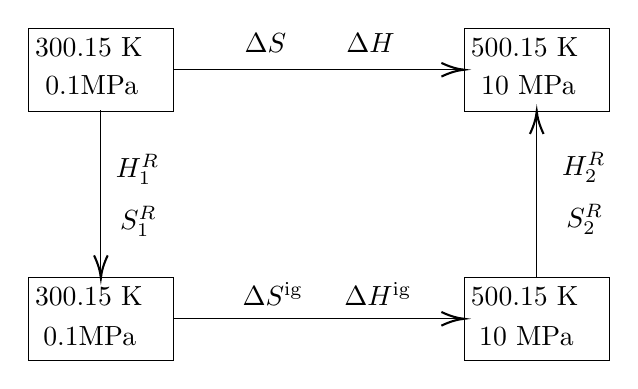
\begin{tikzpicture}[x=0.75pt,y=0.75pt,yscale=-1,xscale=1]
%uncomment if require: \path (0,310); %set diagram left start at 0, and has height of 310

%Shape: Rectangle [id:dp7157481404736188] 
\draw   (138,36) -- (208,36) -- (208,76) -- (138,76) -- cycle ;
%Shape: Rectangle [id:dp4206699841536288] 
\draw   (138,156) -- (208,156) -- (208,196) -- (138,196) -- cycle ;
%Shape: Rectangle [id:dp5931824609872525] 
\draw   (348,36) -- (418,36) -- (418,76) -- (348,76) -- cycle ;
%Shape: Rectangle [id:dp41529041931457367] 
\draw   (348,156) -- (418,156) -- (418,196) -- (348,196) -- cycle ;
%Straight Lines [id:da35176860331240367] 
\draw    (208,56) -- (346,56) ;
\draw [shift={(348,56)}, rotate = 180] [color={rgb, 255:red, 0; green, 0; blue, 0 }  ][line width=0.75]    (10.93,-3.29) .. controls (6.95,-1.4) and (3.31,-0.3) .. (0,0) .. controls (3.31,0.3) and (6.95,1.4) .. (10.93,3.29)   ;
%Straight Lines [id:da0016145845288071392] 
\draw    (208,176) -- (346,176) ;
\draw [shift={(348,176)}, rotate = 180] [color={rgb, 255:red, 0; green, 0; blue, 0 }  ][line width=0.75]    (10.93,-3.29) .. controls (6.95,-1.4) and (3.31,-0.3) .. (0,0) .. controls (3.31,0.3) and (6.95,1.4) .. (10.93,3.29)   ;
%Straight Lines [id:da7326401977633896] 
\draw    (173,75.63) -- (173,154.38) ;
\draw [shift={(173,156.38)}, rotate = 270] [color={rgb, 255:red, 0; green, 0; blue, 0 }  ][line width=0.75]    (10.93,-3.29) .. controls (6.95,-1.4) and (3.31,-0.3) .. (0,0) .. controls (3.31,0.3) and (6.95,1.4) .. (10.93,3.29)   ;
%Straight Lines [id:da20332604498771678] 
\draw    (383,156) -- (383,78) ;
\draw [shift={(383,76)}, rotate = 90] [color={rgb, 255:red, 0; green, 0; blue, 0 }  ][line width=0.75]    (10.93,-3.29) .. controls (6.95,-1.4) and (3.31,-0.3) .. (0,0) .. controls (3.31,0.3) and (6.95,1.4) .. (10.93,3.29)   ;

% Text Node
\draw (140,39.4) node [anchor=north west][inner sep=0.75pt]    {$300.15\ \mathrm{K}$};
% Text Node
\draw (145,57.4) node [anchor=north west][inner sep=0.75pt]    {$\mathrm{0.1MPa}$};
% Text Node
\draw (140,159.4) node [anchor=north west][inner sep=0.75pt]    {$300.15\ \mathrm{K}$};
% Text Node
\draw (144,178.4) node [anchor=north west][inner sep=0.75pt]    {$\mathrm{0.1MPa}$};
% Text Node
\draw (350,39.4) node [anchor=north west][inner sep=0.75pt]    {$500.15\ \mathrm{K}$};
% Text Node
\draw (355,57.4) node [anchor=north west][inner sep=0.75pt]    {$10\ \mathrm{MPa}$};
% Text Node
\draw (354,178.4) node [anchor=north west][inner sep=0.75pt]    {$10\ \mathrm{MPa}$};
% Text Node
\draw (350,159.4) node [anchor=north west][inner sep=0.75pt]    {$500.15\ \mathrm{K}$};
% Text Node
\draw (181,120.4) node [anchor=north west][inner sep=0.75pt]    {$S_{1}^{R}$};
% Text Node
\draw (179,95.4) node [anchor=north west][inner sep=0.75pt]    {$H_{1}^{R}$};
% Text Node
\draw (396,119.4) node [anchor=north west][inner sep=0.75pt]    {$S_{2}^{R}$};
% Text Node
\draw (394,94.4) node [anchor=north west][inner sep=0.75pt]    {$H_{2}^{R}$};
% Text Node
\draw (241,37.4) node [anchor=north west][inner sep=0.75pt]    {$\Delta S$};
% Text Node
\draw (290,37.4) node [anchor=north west][inner sep=0.75pt]    {$\Delta H$};
% Text Node
\draw (240,157.4) node [anchor=north west][inner sep=0.75pt]    {$\Delta S\mathrm{^{ig}}$};
% Text Node
\draw (289,157.4) node [anchor=north west][inner sep=0.75pt]    {$\Delta H^{\mathrm{ig}}$};
\end{tikzpicture}
\end{center}

	$T_{1} = 27+273.15\ \rm{K} = 300.15K$,$T_{2} = 227+273.15\ \rm{K} = 500.15K$,先根据数据计算对比状态:
\begin{equation*}
	T_{r1} = \dfrac{T_1}{T_{c}}=\dfrac{300.15}{417}=0.720
\end{equation*}
\begin{equation*}
	p_{r1} = \dfrac{p_1}{p_{c}}=\dfrac{0.1}{7.701}=0.0130
\end{equation*}

\begin{equation*}
	T_{r2} = \dfrac{T_2}{T_{c}}=\dfrac{500.15}{417}=1.199
\end{equation*}
\begin{equation*}
	p_{r2} = \dfrac{p_2}{p_{c}}=\dfrac{10}{7.701}=1.299
\end{equation*}
这里利用普遍化第二Virial系数法进行计算,首先计算Virial系数:
\begin{equation*}
	B^{0}(T_{r}=0.720)=0.083-\dfrac{0.422}{T_{r}^{1.6}} = 0.083-\dfrac{0.422}{0.720^{1.6}}=-0.631
\end{equation*}
\begin{equation*}
	B^{1}(T_{r}=0.720)=0.139-\dfrac{0.172}{T_{r}^{4.2}} = 0.139-\dfrac{0.172}{0.720^{4.2}}=0.0544
\end{equation*}

\begin{equation*}
	B^{0}(T_{r}=1.199)=0.083-\dfrac{0.422}{T_{r}^{1.6}} = 0.083-\dfrac{0.422}{1.199^{1.6}}=-0.233
\end{equation*}
\begin{equation*}
	B^{1}(T_{r}=1.199)=0.139-\dfrac{0.172}{T_{r}^{4.2}} = 0.139-\dfrac{0.172}{1.199^{4.2}}=0.0587
\end{equation*}
求导都可知:
\begin{equation*}
	\qd{B^{0}}{T_{r}}=\dfrac{0.675}{T_{r}^{2.6}},\quad \qd{B^{0}}{T_{r}}(T_{r}=0.720)=\dfrac{0.675}{0.720^{2.6}} =1.59,\quad \qd{B^{0}}{T_{r}}(T_{r}=1.199)=\dfrac{0.675}{1.199^{2.6}} = 0.421
\end{equation*}
\begin{equation*}
	\qd{B^{1}}{T_{r}}=\dfrac{0.722}{T_{r}^{5.2}},\quad \qd{B^{0}}{T_{r}}(T_{r}=0.720)=\dfrac{0.722}{0.720^{5.2}} = 3.98,\quad \qd{B^{0}}{T_{r}}(T_{r}=1.199)=\dfrac{0.722}{1.199^{5.2}} = 0.281
\end{equation*}
这样直接带入公式即可:
\begin{equation*}
\begin{aligned}
		\dfrac{H^{R}_{1}}{RT}&=p_{r}\pqty{\dfrac{B^{0}}{T_{r}}-\qd{B^{0}}{T_{r}}+\omega\pqty{\dfrac{B^{1}}{T_{r}}-\qd{B^{1}}{T_{r}}}}\\
		&=0.0130\pqty{\dfrac{-0.631}{0.720}-1.59 +0.073\pqty{\dfrac{0.0544}{0.720}-3.98}}\\
		&=-0.358\\
		\dfrac{S^{R}_{1}}{R} &=-p_{r}\pqty{\qd{B^{0}}{R}+\omega\qd{B^{1}}{T_{r}}}\\
		&=-0.0130\pqty{1.59 +0.073\times 3.98}\\
		&=-0.0244
\end{aligned}
\end{equation*}

\begin{equation*}
\begin{aligned}
		\dfrac{H^{R}_{2}}{RT}&=p_{r}\pqty{\dfrac{B^{0}}{T_{r}}-\qd{B^{0}}{T_{r}}+\omega\pqty{\dfrac{B^{1}}{T_{r}}-\qd{B^{1}}{T_{r}}}}\\
		&=1.299\pqty{\dfrac{-0.233}{1.199}-0.421+0.073\pqty{\dfrac{0.0587}{1.199}-0.281}}\\
		&=-0.821\\
		\dfrac{S^{R}_{2}}{R} &=-p_{r}\pqty{\qd{B^{0}}{R}+\omega\qd{B^{1}}{T_{r}}}\\
		&=-1.299\pqty{0.421 +0.073\times 0.281}\\
		&=-0.574
\end{aligned}
\end{equation*}

这样一来,移项即可求得:
\begin{equation*}
	H^{R}_{1} = -89.3{\rm{J}\cdot\rm{mol}^{-1}}\quad S^{R}_{1}=0.203\rm{J}\cdot\rm{mol}^{-1}\cdot\rm{K}^{-1}
\end{equation*}
\begin{equation*}
	H^{R}_{2} = -3415{\rm{J}\cdot\rm{mol}^{-1}}\quad S^{R}_{2}=-4.768\rm{J}\cdot\rm{mol}^{-1}\cdot\rm{K}^{-1}
\end{equation*}
对于理想气体的变温变压过程,根据化学热力学中的公式可知:
\begin{equation*}
\begin{aligned}
	\Delta H^{{\rm{ig}}}&=\int_{T_{1}}^{T_{2}}C_{p}^{{\rm{ig}}}{\rm{d}}T =\int_{300.15}^{500.15}(31.696+10.144\times 10^{-3}T-4.038\times 10^{-6}T^{2}){\rm{d}}T =7019{\rm{J}\cdot\rm{mol}^{-1}}\\
		\Delta S^{{\rm{ig}}}&=\int_{T_{1}}^{T_{2}}\dfrac{C_{p}^{{\rm{ig}}}}{T}{\rm{d}}T+R\ln{\dfrac{p_{1}}{p_{2}}}=\int_{300.15}^{500.15}\dfrac{31.696+10.144\times 10^{-3}T-4.038\times 10^{-6}T^{2}}{T}{\rm{d}}T+8.314\ln{\dfrac{0.1}{10}}\\
		&=-20.4\rm{mol}^{-1}\cdot\rm{K}^{-1}
\end{aligned}
\end{equation*}
综上,整个过程的焓、熵变化为:
\begin{equation*}
	\begin{aligned}
		\Delta H &= -H^{R}_{1}+\Delta H^{{\rm{ig}}}+H^{R}_{2}=89.3+7019-3415\ {\rm{J}\cdot\rm{mol}^{-1}}= 3693.3 {\rm{J}\cdot\rm{mol}^{-1}}\\
		\Delta S &= -S^{R}_{1}+\Delta S^{{\rm{ig}}}+S^{R}_{2}=  -0.203-20.4-4.768\ \rm{mol}^{-1}\cdot\rm{K}^{-1} = -25.071\rm{mol}^{-1}\cdot\rm{K}^{-1}\\
	\end{aligned}
\end{equation*}

\end{solution}



\begin{problem}
	试采用RK方程计算在227\ssd、5MPa下的气相正丁烷的剩余焓和剩余熵。正丁烷的临界参数和偏心因子分别为:
$T_{c}$=425.2K ,$p_{c}$=3.800MPa ,$\omega$=0.193
\end{problem}

\begin{solution}
	$T = 227+273.15 \ \rm{K} = 500.15\rm{K}$,利用R-K方程,先计算物性常数:
	\begin{equation*}
		a = 0.42748\dfrac{R^{2}T_{c}^{2.5}}{p_{c}} = 0.42748\dfrac{8.314^{2}\times 425.2^{2.5}}{3.800}\rm{Pa}\cdot \rm{K}^{0.5}\cdot\rm{m}^{6}\cdot\rm{Mmol}^{-2}=29.0\rm{Pa}\cdot \rm{K}^{0.5}\cdot\rm{m}^{6}\cdot\rm{mol}^{-2}
	\end{equation*}
	\begin{equation*}
			b = 0.08664\times\dfrac{RT_{c}}{p_{c}} = 0.08664\times\dfrac{8.314\times 425.2}{3.800}\rm{m}^{3}\cdot\rm{Mmol}^{-1}=8.06\times 10^{-5}\rm{m}^{3}\cdot\rm{mol}^{-1}
	\end{equation*}
	然后列出R-K方程:
	\begin{equation}
		p  = \dfrac{RT}{V-b}-\dfrac{a}{T^{0.5}V(V+b)} 
	\end{equation}
	然后利用计算机解之\footnote{利用Patrick Barrie's program for solving cubic equations of state,具体网址在\href{http://www.mathaddict.net/realgas4.htm}{http://www.mathaddict.net/realgas4.htm}} ,得到:
	\begin{equation*}
		V_{m} = 0.000570{\rm{m}}^{3}\cdot{\rm{mol}}^{-1}
	\end{equation*}
	然后带入公式即可求出:
	\begin{equation*}
		\begin{aligned}
			H^{R} &=pV_{m}-RT-\dfrac{3a}{2T^{0.5}b}\ln{\pqty{1+\dfrac{b}{V_{m}}}} \\
			&=5\times 10^{6}\times 0.000570 -8.314\times 500.15-\dfrac{3\times 29.0}{2\times 500.15^{0.5}\times 8.06\times 10^{-5}}\ln{\pqty{1+\dfrac{8.06\times 10^{-5}}{0.000570}}} \\
			&=-4500 {\rm{J}\cdot\rm{mol}^{-1}}\\
			S^{R} &= R\ln{(V_{m}-b)}-R\ln{\dfrac{RT}{p}}-\dfrac{a}{2T^{1.5}b}\ln{\pqty{1+\dfrac{b}{V_{m}}}}\\
	&= 8.314\ln{(0.000570-8.06\times 10^{-5})}-8.314\ln{\dfrac{8.314\times 500.15}{5\times 10^{6}}}\\
	&\quad \quad \quad -\dfrac{29.0}{2\times 500.15^{1.5}\times 8.06\times 10^{-5}}\ln{\pqty{1+\dfrac{8.06\times 10^{-5}}{0.000570}}}=-6.54\rm{mol}^{-1}\cdot\rm{K}^{-1}
		\end{aligned}
	\end{equation*}
\end{solution}

\begin{problem}
	假设125\ssd、10MPa下的丙烯服从R-K状态方程,试运用 R-K 方程求算该状态下的丙烯的剩余焓与剩余熵。该状态下的丙烯的$V_{m} = 1.42\times 10^{-4}\rm{m}^{3}\cdot \rm{mol}$,丙烯的临界参数和偏心因子分别为:
$T_{c}$=3650K , $p_{c}$=4.620MPa , $\omega$=0.193

\end{problem}
\begin{solution}
	$T = 125+273.15\ \rm{K} = 398.15\rm{K}$利用R-K方程,还是先计算物性常数:
	\begin{equation*}
		a = 0.42748\dfrac{R^{2}T_{c}^{2.5}}{p_{c}} = 0.42748\dfrac{8.314^{2}\times 365.0^{2.5}}{4.620}\rm{Pa}\cdot \rm{K}^{0.5}\cdot\rm{m}^{6}\cdot\rm{Mmol}^{-2}=16.28\rm{Pa}\cdot \rm{K}^{0.5}\cdot\rm{m}^{6}\cdot\rm{mol}^{-2}
	\end{equation*}
	\begin{equation*}
			b = 0.08664\times\dfrac{RT_{c}}{p_{c}} = 0.08664\times\dfrac{8.314\times 365.0}{4.620}\rm{m}^{3}\cdot\rm{Mmol}^{-1}=5.691\times 10^{-5}\rm{m}^{3}\cdot\rm{mol}^{-1}
	\end{equation*}
	如上题,同样得到:
	\begin{equation*}
		V_{m} = 0.0001360{\rm{m}}^{3}\cdot{\rm{mol}}^{-1}
	\end{equation*}
	然后带入公式即可求出:
	\begin{equation*}
		\begin{aligned}
			H^{R} &=pV_{m}-RT-\dfrac{3a}{2T^{0.5}b}\ln{\pqty{1+\dfrac{b}{V_{m}}}} \\
			&=10\times 10^{6}\times 0.0001360 -8.314\times 398.15-\dfrac{3\times 16.28}{2\times 398.15^{0.5}\times 5.691\times 10^{-5}}\ln{\pqty{1+\dfrac{5.691\times 10^{-5}}{0.0001360}}} \\
			&= -9468 {\rm{J}\cdot\rm{mol}^{-1}}\\
		\end{aligned}
	\end{equation*}
	\begin{equation*}
		\begin{aligned}
			S^{R} &= R\ln{(V_{m}-b)}-R\ln{\dfrac{RT}{p}}-\dfrac{a}{2T^{1.5}b}\ln{\pqty{1+\dfrac{b}{V_{m}}}}\\
	&= 8.314\ln{(0.0001360-5.691\times 10^{-5})}-8.314\times\ln{\dfrac{8.06\times 10^{-5}\times 398.15}{10\times 10^{6}}}\\
	&\quad \quad \quad -\dfrac{16.28}{2\times 398.15^{1.5}\times5.691\times 10^{-5}}\ln{\pqty{1+\dfrac{5.691\times 10^{-5}}{0.0001360}}}=-18.20\rm{mol}^{-1}\cdot\rm{K}^{-1}
		\end{aligned}
	\end{equation*}
\end{solution}
\chapter{2022年4月14日\quad 晴$^{\star}$}
本次作业的第一题是上一次作业的倒数第二题,剩下两题解答如下:
\begin{problem}
	试用普遍化方法计算二氧化碳在473.2K、30MPa下的焓与熵。二氧化碳的临界参数和偏心因子分别为:
$T_{c}=304.2\ce{K},p_{c}=7.376{\rm{MPa}},\omega =0.225$。已知在相同条件下,二氧化碳处于理想状态的焓为$8377\rm{J}\cdot\rm{mol}^{-1}$,熵为$-25.86\rm{J}\cdot\rm{mol}^{-1}\cdot\rm{K}^{-1}$。
\end{problem}
\begin{solution}
先根据数据计算对比状态:
\begin{equation*}
	T_{r} = \dfrac{T}{T_{c}}=\dfrac{473.2}{304.2}=1.556
\end{equation*}
\begin{equation*}
	p_{r} = \dfrac{p}{p_{c}}=\dfrac{30}{7.376}=4.067
\end{equation*}
然后计算Virial系数:
\begin{equation*}
	B^{0}(T_{r}=1.556)=0.083-\dfrac{0.422}{T_{r}^{1.6}} = 0.083-\dfrac{0.422}{1.556^{1.6}}=-0.125
\end{equation*}
\begin{equation*}
	B^{1}(T_{r}=1.556)=0.139-\dfrac{0.172}{T_{r}^{4.2}} = 0.139-\dfrac{0.172}{1.556^{4.2}}=0.112
\end{equation*}
求导可知:
\begin{equation*}
	\qd{B^{0}}{T_{r}}=\dfrac{0.675}{T_{r}^{2.6}},\quad \qd{B^{0}}{T_{r}}(T_{r}=1.556)=\dfrac{0.675}{1.556^{2.6}} =0.214
\end{equation*}
\begin{equation*}
	\qd{B^{1}}{T_{r}}=\dfrac{0.722}{T_{r}^{5.2}},\quad \qd{B^{0}}{T_{r}}(T_{r}=1.556)=\dfrac{0.722}{1.556^{5.2}} = 0.0725
\end{equation*}
这样直接带入公式即可:
\begin{equation*}
\begin{aligned}
		\dfrac{H^{R}}{RT}&=p_{r}\pqty{\dfrac{B^{0}}{T_{r}}-\qd{B^{0}}{T_{r}}+\omega\pqty{\dfrac{B^{1}}{T_{r}}-\qd{B^{1}}{T_{r}}}}\\
		&=4.067\pqty{\dfrac{-0.125}{1.556}-0.214 +0.225\pqty{\dfrac{0.112}{1.556}-0.0725}}\\
		&=-1.197\\
\end{aligned}
\end{equation*}
\begin{equation*}
\begin{aligned}
		\dfrac{S^{R}}{R} &=-p_{r}\pqty{\qd{B^{0}}{R}+\omega\qd{B^{1}}{T_{r}}}\\
		&=-4.067\pqty{0.214+0.225\times 0.0725}\\
		&=-0.9367
\end{aligned}
\end{equation*}
这样就可以得到:
\begin{equation*}
\begin{aligned}
	H(473.2\ce{K},30\ce{MPa}) &= H^{R}+H^{\ce{ig}}(473.2\ce{K},30\ce{MPa})\\
	&=-1.197\times 8.314\times 473.2+8377\ \rm{J}\cdot\rm{mol}^{-1}\\
	&=3668\rm{J}\cdot\rm{mol}^{-1}\\
	S(473.2\ce{K},30\ce{MPa})&= S^{R}+S^{\ce{ig}}(473.2\ce{K},30\ce{MPa})\\
	&=-0.9367\times 8.314-25.86 \ \rm{J}\cdot\rm{mol}^{-1}\cdot\rm{K}^{-1}\\
	&=-33.65\rm{J}\cdot\rm{mol}^{-1}\cdot\rm{K}^{-1}
\end{aligned}
\end{equation*}

\end{solution}


\begin{problem}
	试用普遍化第二维里系数法计算丙烷气体在378K、0.507MPa下的剩余焓。已知丙烷的临界常数:$T_{c}=369.8\ce{K},p_{c}=4.246{\rm{MPa}},\omega =0.152$。
\end{problem}
\begin{solution}
先根据数据计算对比状态:
\begin{equation*}
	T_{r} = \dfrac{T}{T_{c}}=\dfrac{378}{369.8}=1.02
\end{equation*}
\begin{equation*}
	p_{r} = \dfrac{p}{p_{c}}=\dfrac{0.507}{4.246}=0.119
\end{equation*}
然后计算Virial系数:
\begin{equation*}
	B^{0}(T_{r}=1.02)=0.083-\dfrac{0.422}{T_{r}^{1.6}} = 0.083-\dfrac{0.422}{1.02^{1.6}}=-0.326
\end{equation*}
\begin{equation*}
	B^{1}(T_{r}=1.02)=0.139-\dfrac{0.172}{T_{r}^{4.2}} = 0.139-\dfrac{0.172}{1.02^{4.2}}=-0.0162
\end{equation*}
求导可得:
\begin{equation*}
	\qd{B^{0}}{T_{r}}=\dfrac{0.675}{T_{r}^{2.6}},\quad \qd{B^{0}}{T_{r}}(T_{r}=1.02)=\dfrac{0.675}{1.02^{2.6}} =0.641
\end{equation*}
\begin{equation*}
	\qd{B^{1}}{T_{r}}=\dfrac{0.722}{T_{r}^{5.2}},\quad \qd{B^{0}}{T_{r}}(T_{r}=1.02)=\dfrac{0.722}{1.02^{5.2}} = 0.651
\end{equation*}
这样直接带入公式即可:
\begin{equation*}
\begin{aligned}
		\dfrac{H^{R}}{RT}&=p_{r}\pqty{\dfrac{B^{0}}{T_{r}}-\qd{B^{0}}{T_{r}}+\omega\pqty{\dfrac{B^{1}}{T_{r}}-\qd{B^{1}}{T_{r}}}}\\
		&=0.119\pqty{\dfrac{-0.326}{1.02}-0.641 +0.152\pqty{\dfrac{-0.0162}{1.02}-0.651}}\\
		&=-0.126\\
		\dfrac{S^{R}}{R} &=-p_{r}\pqty{\qd{B^{0}}{R}+\omega\qd{B^{1}}{T_{r}}}\\
		&=-0.119\pqty{0.641+0.152\times 0.651}\\
		&=-0.0881\\
\end{aligned}
\end{equation*}
这样就得到:\begin{equation*}
	H^{R} = -397{\rm{J}\cdot\rm{mol}^{-1}}, \quad S^{R} = 0.732\rm{J}\cdot\rm{mol}^{-1}\cdot\rm{K}^{-1}
\end{equation*}
\end{solution}



\chapter{2022年4月21日\quad 晴$^\dag$}
\begin{problem}
	某容器内的液态水和蒸汽在1MPa下处于平衡状态,质量为1kg。假如容器内液体和蒸汽各占一半体积,试求容器内的液态水和蒸汽的总焓。
	
已知:饱和水蒸汽表,1MPa时,$H_{l} = 762.81{\rm{kJ}}\cdot{\rm{kg}}^{-1}$、$H_{g} = 2778.1{\rm{kJ}}\cdot{\rm{kg}}^{-1}$、$V_{l} = 1.1273{\rm{cm}}^{3}\cdot{\rm{g}}^{-1}$、$V_{g} = 194.4{\rm{cm}}^{3}\cdot{\rm{g}}^{-1}$
\end{problem}
\begin{solution}
	设水饱和蒸汽占全体的质量比重\footnote{也叫\textcolor{myblu}{干度},这里不这么称呼是为了减少边缘名词个数}为$x$,这样就可以根据体积相等给出以下关系式:
	\begin{equation*}
		xV_{g} = (1-x)V_{l}
	\end{equation*}
	代入数据,可得:
	\begin{equation*}
		194.4x=1.1273(1-x)
	\end{equation*}
	解得$x = 0.005765$
那么体系的总焓$H$可以表示为以下式子:
	\begin{equation*}
		\begin{aligned}
			H &=(1-x)H_{l}+ xH_{g}\\
			&=(1-0.005765)\times 762.81+0.005765\times 2778.1\  {\rm{kJ}}\cdot{\rm{kg}}^{-1} = 774.43{\rm{kJ}}\cdot{\rm{kg}}^{-1}
		\end{aligned}
	\end{equation*}
\end{solution}




\begin{problem}
	假设二氧化碳服从RK状态方程,计算50\ssd、10.13MPa时二氧化碳的逸度。二氧化碳的临界参数和偏心因子分别为:$T_{c}$=304.2K,$p_{c}$=7.376MPa,$\omega$=0.225
\end{problem}

\begin{solution}
	先计算物性常数:
	\begin{equation*}
		a = 0.42748\dfrac{R^{2}T_{c}^{2.5}}{p_{c}} = 0.42748\times\dfrac{8.314^{2}304.2^{2.5}}{7.376}\rm{Pa}\cdot \rm{K}^{0.5}\cdot\rm{m}^{6}\cdot\rm{Mmol}^{-1}= 6.466\rm{Pa}\cdot \rm{K}^{0.5}\cdot\rm{m}^{6}\cdot\rm{mol}^{-1}
	\end{equation*}
	\begin{equation*}
		b = 0.08664\times\dfrac{RT_{c}}{p_{c}} = 0.08664\times\dfrac{8.314\times 304.2}{7.376}\rm{m}^{3}\cdot\rm{Mmol}^{-1}= 29.71\times 10^{-6}\rm{m}^{3}\cdot\rm{mol}^{-1}
	\end{equation*}


待求温度为$T = 50+273.15\ \rm{K} = 323.15\rm{K}$,然后列出R-K方程,并反解\footnote{仍然利用Patrick Barrie's program for solving cubic equations of state,具体网址在\href{http://www.mathaddict.net/realgas4.htm}{http://www.mathaddict.net/realgas4.htm}}得:$V_{m} = 0.0001082\rm{m}^{3}\cdot\rm{mol}^{-1}$此时压缩因子为$Z = 0.4079$


然后带入逸度因子的求算公式得到:
\begin{equation*}
	\begin{aligned}
		\ln{\varphi} = \ln{\dfrac{f}{p}} &= Z-1-\ln(Z - \dfrac{bp}{RT})-\dfrac{a}{bRT^{1.5}}\ln(1+\dfrac{b}{V_{m}})\\
		&=0.4079-1-\ln(0.4079 - \dfrac{29.71\times 7.376}{8.314\times 304.2})\\
		&-\dfrac{6.466}{29.71\times 10^{-6}\times 8.314\times 323.15^{1.5}}\ln(1+\dfrac{29.71\times 10^{-6}}{0.0001082})\\
		&=-0.6536
	\end{aligned}
\end{equation*}
这样就可知:
\begin{equation*}
	f = p\times e^{-0.6536} = 7.376\times e^{-0.6536} \rm{MPa}=3.837MPa
\end{equation*}
\end{solution}
\begin{problem}
试计算液态水在30\ssd 下,压力分别为(a)饱和蒸气压(b)$100\times 10^{5}$Pa下的逸度和逸度系数。
已知:
\begin{enumerate}
	\item 水在30\ssd 时的饱和蒸气压$p^{s} = 0.0424\times 10^{5}$Pa。
	\item 30\ssd ,$0\sim 100\times 10^{5}$Pa范围内将液态水的摩尔体积视为常数,其值为$0.01809 {\rm{m}}^{3}\cdot {\rm{kmol}}^{-1}$。
	\item $100\times 10^{5}$Pa以下的水蒸气可以视为理想气体。
\end{enumerate}
\end{problem}


\begin{solution}
	\begin{enumerate}
		\item[(a)] 当此之时,30\ssd 液态水之气压为饱和蒸气压,故其处于相平衡状态;又由于其压力较小,饱和水蒸气视作理想气体,故$f = p^{s} =0.0424\times 10^{5}\ce{Pa},\ \varphi = 1$
		\item[(b)] 此时压力$p = 100\times 10^{5}\rm{Pa}$,所以不再处于相平衡状态。那么:
		\begin{equation*}
			\begin{aligned}
				\ln{\varphi} = \ln{\dfrac{f}{p}} &= \int_{p^{s}}^{p} \pqty{\dfrac{V_{m}}{RT} - \dfrac{1}{p}}\ce{d}p\\
				&=\int_{0.0424\times 10^{5}{\rm{Pa}}}^{100\times 10^{5}\ce{Pa}}\pqty{\dfrac{0.01809\times 10^{-3}{\rm{m}}^{3}\cdot {\rm{mol}}^{-1}}{8.314\times (273.15+30)\ce{Pa}\cdot\ce{m}^{3}\cdot\ce{mol}^{-1}}-\dfrac{1}{p}}\ce{d}p\\
				&=-7.694
			\end{aligned}
		\end{equation*}
		明显有$\varphi = e^{-7.694} = 0.0004555$,且有:
		\begin{equation*}
			f = p\times e^{-7.694} = 100\times 10^{5}\times e^{-7.694}\ce{Pa} = 4555\ce{Pa}
		\end{equation*}
	\end{enumerate}
\end{solution}








\end{document}